\documentclass[12pt,english]{rftthesis}

\usepackage[utf8]{inputenc}
\usepackage[T1]{fontenc}
\usepackage[nottoc]{tocbibind}
\usepackage{csquotes}
\usepackage{svg}
\usepackage{setspace}
\usepackage{float}
\usepackage{caption}
\usepackage{hyperref}
\usepackage{wrapfig}
\usepackage{inconsolata}
\usepackage[toc,page]{appendix}
\usepackage{framed}
\usepackage{quoting}
\usepackage{underscore}
\usepackage{xcolor}
\usepackage{tcolorbox}
\usepackage{graphicx,calc}
\usepackage{tabularx}
\usepackage{array}
\usepackage{enumitem}
\usepackage{soul}
\usepackage{booktabs}
\usepackage{makecell}
\usepackage{subcaption}
\usepackage[cache=false]{minted}
\tcbuselibrary{minted,skins}

\title           	{Development of a Snapshotting Technique within Dream Chaser's Software-in-the-loop Test Framework}
\type            	{Masters thesis}
\author          	{B.Eng. Alexis Cabana-Loriaux}
\matriculation   	{0407200}
\studies         	{Masters of Space Engineering}
\firstsupervisor 	{Prof. Dr.-Ing. Klaus Brieß}
\secondsupervisor	{M.Sc. Mario Starke}
\industrysupervisor {Claudio Discepola, Senior Member, MDA Corporation}
\date            	{\today}


% Glossary is defined in preamble
\makenoidxglossaries
\setacronymstyle{long-short}

\newacronym{DCCS}{DCCS}{Dream Chaser Cargo System}
\newacronym{SNC}{SNC}{Sierra Nevada Corporation}
\newacronym{ISS}{ISS}{International Space Station}
\newacronym{NASA}{NASA}{National Aeronautics and Space Administration}
\newacronym{CRS}{CRS}{Commercial Resupply Services}
\newacronym{CCDev}{CCDev}{Commercial Crew Development}
\newacronym{LEO}{LEO}{Low-Earth Orbit}
\newacronym{MDA}{MDA}{MacDonald, Dettwiler and Associates Ltd.}
\newacronym{DCMS}{DCMS}{Dream Chaser Mission Simulator}
\newacronym{SIL}{SIL}{software-in-the-loop}
\newacronym{BBPSim}{BBPSim}{Baseband Processor Simulator}
\newacronym{FSW}{FSW}{flight software}
\newacronym{VM}{VM}{virtual machine}
\newacronym{VMM}{VMM}{virtual machine monitor}
\newacronym{FPU}{FPU}{Floating-point Unit}
\newacronym{MMU}{MMU}{Memory Management Unit}
\newacronym{SLAT}{SLAT}{Second Level Address Translation }



% references are also defined in preamble
\addbibresource{ref/references.bib}

%add custom commands
\newcommand{\source}[1]{\caption*{\textbf{Source:} {#1}} }


\begin{document}
%First page here
%\maketitle
%\makedeclaration
\onehalfspacing

{ 
% pre-thesis content
%\chapter*{Acknowledgements}\label{cha:ack}
This thesis is by far the most interesting project I've ever had to work on in my young career. Never would I have thought I would be working on such an impressive private spacecraft project as part of my studies. 

As such, I would like to thank my program managers Guillaume Lemieux and François Arsenault for their trust and for having given me the green light. A huge thank you to the whole Dream Chaser team at MDA is also in order. They supported me very well, even with the home office situation. Precisely, I would like to mention my team leads Claudio Discepola and Fatima Zahra Tazi, my technical mentor Martin Servant, as well as Matthieu Ippersiel and Frederic Lamer, who seemed to always hold the solutions to my bizarre problems.

Finally, I would also like to thank my TU Berlin supervisor, M.Sc. Mario Starke, for guiding me and providing valuable feedback. 

%\chapter*{Abstract}\label{cha:abstract}
indirectly deducing variable addresses of a dynamically linked library at runtime  by taking advantage of build time to embed raw bytes. linktwice
%\chapter*{Résumé}\label{cha:resume}
La simulation fonctionnelle forme une partie intégrante de la phase de test des projets de systèmes spatiaux. Pour le sous-système de communication du vaisseau spatial Dream Chaser, une fonction de type \textit{snapshot} a dû être développée pour son système de test logiciel-dans-la-boucle, similairement à des programmes de virtualisation. En utilisant des concepts existants, cette thèse démontre comment un instantané du logiciel de vol a pu être effectué, sans modifier son code, à travers l'injection de code visant à enregistrer l'état de ses fils d'exécution et en cataloguant ses variables entre deux éditions des liens. Après la production d'un artefact au format défini, l'environement de test a pu être entièrement restauré en manipulant les cadres de piles d'exécution pour reconstruire les fils de vol, parallèlement à la reconstruction des modules de simulation. Des résultats sont ensuite présentés pour démontrer la conformité de la fonctionalité aux requis de performance du client.
%\chapter*{Zusammenfassung}\label{cha:zusammenfassung}

}

%\tableofcontents

%\listoftables

%\listoffigures

%\listoflistings

%\printnoidxglossary[type=acronym,nonumberlist]
{
% Whole content of the thesis
%\setlength{\parindent}{2em}
\chapter{Introduction}\label{cha:intro}
\pagenumbering{arabic}
Since the termination of the Space Shuttle program in 2011, the \gls{NASA} has been turning to other countries and private enterprises for the transportation of cargo to orbit and beyond. The \gls{CRS} program is a good example of this: a public-private partnership in which supplies provided by NASA are launched into orbit to the \gls{ISS} by commercial rockets. Of course, the new "Delivery-as-a-Service" paradigm has spawned a lot of commercial interest all around the world. In the United States, the Dream Chaser program is one of those efforts that continue strengthening the ties between public space agencies and the private sector.

\section{The Dream Chaser program}
This thesis' scope is entirely contained within the Dream Chaser project. Therefore, the spacecraft and its design is the main subject. 
\subsection*{History}
Conceptualized in 2004 by SpaceDev, the \gls{DCCS} program was officially kick-started by \gls{SNC} in 2010, following its acquisition of SpaceDev in 2008\cite{online:fikes}. Seeing the potential and future possibilities of the transportation system, NASA then awarded funding for the project as part of their \gls{CCDev} program, furthering the development efforts. As \gls{SNC} started breaking down the spacecraft into several sub-systems, it also started subcontracting their development to other companies. So far, the first flight to the \gls{ISS} is officially scheduled to take place in late 2021\cite{online:kanayama}.

\subsection*{Features}
The \gls{DCCS} is an unmanned, reusable orbital spaceplane intended for the transportation of both pressurized and unpressurized cargo to and from the \gls{ISS}. It contains many features that make it a very interesting solution for different kinds of space needs. 

First of all, the system contains a powerful propulsion system made out of a cluster of Orbitec's Vortex engines\cite{online:messier}. This enables self-cruising and orbit correction, instead of being 100\% reliant on the launch provider for exact orbit insertion. Furthermore, this on-board propulsion opens up other possibilities for Dream Chaser deeper than \gls{LEO}, like transporting cargo to the coming Lunar Gateway\cite{online:foust}.

Secondly, the  spacecraft is partly made reusable by the development of a custom, very resistant airframe by Lockheed Martin. The haul, its wings and landing gear enable \gls{DCCS} to safely land on a runway from \gls{LEO}. These features make Dream Chaser physically comparable to a Space Shuttle (see \autoref{fig:dccs-landed}). 
\begin{figure}[H]
	\centering
	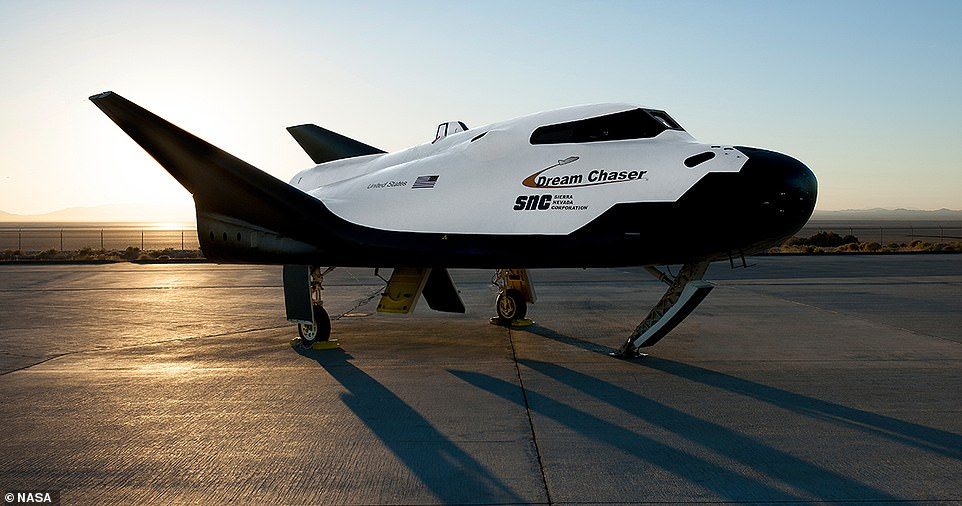
\includegraphics[width=0.9\linewidth, keepaspectratio]{art/dream-chaser-landed.jpg}
	\caption{Dream Chaser on a runway at sunset \cite{misc:dccs-landed}}
	\label{fig:dccs-landed}
\end{figure}
Finally, its communication subsystem is made of several types of antennas, for encrypted telecommunication with ground stations and the \gls{ISS}. Because docking to the space station is also one of the spacecraft's capabilities, a physical communication link is present too. \gls{MDA} has been put in charge of this crucial component's development by \gls{SNC}. 

\section{MDA - Industry partner}
\gls{MDA} is one of the greatest actors in the emerging Canadian space industry. In 2018, it composed nearly one-fifth of the total number of space sector jobs in the country\cite{online:mda-front-page}\cite{misc:canada-space-industry-report}. The Canada-based company, which has offices in Montreal, has already partnered on multiple occasions with the Canadian Space Agency. It's most notable contributions are the design and manufacturing of the Canadarm2 on the \gls{ISS}, as well as the RADARSAT-2 satellite constellation. This thesis was made in partnership with \gls{MDA}, in the context of a 6 months thesis-internship in Montreal during which the present project was scoped, planned and executed. The work was officially supervised by Claudio Discepola, Senior member of the Dream Chaser team. 

\section{Background}\label{sec:intro-background}
With the ever decreasing cost of computing power, functional simulation of components and systems has become an integral part of the testing phase in space design. This approach is thus also taken by \gls{SNC} in the context of Dream Chaser, who requires subcontractors like \gls{MDA} to provide simulators of their respective subsystems alongside the subsystem itself. This is done with the intent of simulating, on multiple fronts, an entire launch or mission, from the reception and handling of telecommands to the behavior of the flight computer mid-mission. 

Once the simulators are all working separately, they are then interfaced together. This results in a compute-intensive platform called the \gls{DCMS}, an important piece in the integration, testing and validation phases of the development. By its virtual nature, the \gls{DCMS} can be ran under different conditions in order to observe the behavior of the spacecraft as a whole in different scenarios. This proves to be  very useful, for example, in the early detection of anomalies or also in the regression testing of software.

Each subcontractor's simulator possesses its own set of requirements, driven by the desired simulation quality and granularity. In that sense, \gls{MDA} is in charge of developing the \gls{BBPSim}, a \gls{SIL} platform for the flight code of the entire communication subsystem, from the antennas to the computing nodes themselves. \gls{BBPSim} acts as some sort of hypervisor, exposing an interface to operating system and hardware utilities to the flight software, itself fundamentally written for an embedded platform. This makes abstraction of the system on which the code is running while keeping all of its functionalities and internal algorithms. As a result, \gls{BBPSim} significantly improves the easiness of interaction with the flight software as well as enabling its testing on a Linux machine in a continuous integration pipeline system like Jenkins.

\section{Purpose}
The purpose of this thesis is to design and develop a custom-fit \textit{snapshotting} technique for \gls{BBPSim}. As said previously, the development of the simulator is driven by the requirements derived from its inclusion in the DCMS. The need for a snapshot feature comes from a pair of them, that state that
\begin{enumerate}
	\item \gls{BBPSim} shall have the capability of saving its state, or "context", to non-volatile memory.
	\item \gls{BBPSim} shall be able to restore itself from a state file in non-volatile memory at initialization.
\end{enumerate} 

This snapshotting feature (often called the \textit{Save \& restore} in the document) will be a considerable addition to the \gls{BBPSim} framework. It will add the possibility to exhaustively represent an on-going simulation at a definite time $t$. It is called a snapshot due to its many similarities with virtual machine software like the open-source VirtualBox. In VirtualBox, it is possible for the user to pause, or to "snapshot" a running instance of a virtual machine, to save it into a relatively large file (called state file) and to restore everything back exactly like it was: running programs, graphics card output and general OS state are all recovered.  

Save \& restore has considerable advantages from a testing point of view. For instance, in the context of Dream Chaser, the flight software enters different states depending on the phase of launch the spacecraft is in. The code doesn't have the same behavior during the launch phase than it has when in the docking phase. However, for the software to change state, some sort of outside stimuli must happen. This external manipulation, albeit automatically executed, can last many minutes for each test. Considering there are hundreds of tests, the time for exhaustive regression testing is of course significant. The snapshot feature completely removes that limitation, because it enables the simulator to be instantly started to a previous state without having to interact with the \gls{FSW}. It is possible to shortcut directly to the docking phase without having to go trough simulating the launch phase. 

Furthermore, another benefit of the feature is that it allows the same hypothetical failures to be replayed over and over again. Since a state file can be restored again and again at will, the interaction between all the different subsystems can be analyzed more in-depth. When in the integration phase, potential inter-system faults can be caught earlier and they are easier to reproduce.  

\section{Thesis Overview TO BE UPDATED}
This thesis will start by giving an general idea of such a \textit{snapshotting} concept in the context of other software projects. There has been many successful attempts to create this mechanism in academic papers and open-source programs, instances from which inspiration has been drawn. Then, the design and implementation of the feature inside \gls{BBPSim} is discussed in details. The general approach in terms of changing the simulator's software to make it saveable is explained. After these crucial steps, the integration of the work in the existing testing pipeline as well as its impact on the testing process at MDA are also covered. 

The rest of this paper is organized as follows. In Section 2, we present background
for and define the problem. In Section 3, we define some terminology and describe
our basic approach. In Section 4, we discuss some of the difficulties of adding faulttolerance to MPI programs. In Sections 5 and 6 we present non-blocking checkpointing
protocols for point-to-point and collective communication, respectively. In Section 7,
we discuss how our system saves the sequential state of each process. In Section 8, we
present performance results of our system. In Section 9 we discuss related work, and in
Section 10 we describe future work. In Section 11, we offer some conclusions.

%{
\setlength{\parindent}{2em}
\chapter{Software Environment}\label{cha:sim-env}
Before proceeding to any design, it was important to first thoroughly characterize the setting in which the save \& restore was implemented. Fundamentally, this thesis was an integration project and, without a surprise, the checkpointing feature had to be merged coherently in the previously existing environment.

This chapter better describes the main driving factors in the design of the feature. From user and customer requirements to technical considerations, it serves as the basis on which everything was subsequently built.

\section{Requirements}
In the context of the \gls{DCCS}, Sierra Nevada Corporation subcontracted the entire design and implementation of the communications subsystem to \gls{MDA}. \gls{SNC} had clear goals with Dream Chaser, and for this multi-company undertaking to be properly organized, a hierarchical list of requirements had to be produced. The list was then given to the relevant subcontractors so they could guide themselves in the design of their subsystem. The final product could then be analyzed to assess how well it met the expectations. 

In the Dream Chaser program, the main product to be delivered by \gls{MDA} was the \gls{BBP} along with \gls{DAS}, its flight software. However, even though \gls{BBPSim} was treated as a sub-product to be delivered in conjunction, it also possessed its own set of requirement documents.

In the case of this thesis, two types of requirements were driving factors in the design, each with a different scope. Of course, the primary customer requirements from \gls{SNC} had to be followed, but another set was produced in parallel to provide additional guidelines to help the fulfillment of the feature.  

\subsection*{Customer Requirements}
\textit{Scope: the {BBPSim} framework.}

Throughout the thesis work, the customer requirements of the entire \gls{BBPSim} ecosystem were taken as the main drivers to follow for the development. As a measure of legal prudence, the integral list of requirements cannot be made available in this document. \autoref{tab:customer-reqs} lists several of them that relate to the development of the checkpointing feature.  
\begin{table}[htbp]
	\vspace{12pt}
	\centering
	\ra{1.3}
	\begin{tabularx}{\linewidth}{>{\centering}p{3cm} X}
		\toprule
		{\bfseries Requirement\newline Number} & \textbf{Description}\\
		\midrule
		DCMS-BBP-32 & {The BBP Simulator software shall support real-time (RT) execution whereby BBP FSW tasks are executed at the rate they would be on actual BBP hardware.}\\
		\midrule
		DCMS-BBP-53 & {The BBP Simulator software shall provide the capability to initialize, step, and terminate.}\\
		\midrule
		DCMS-BBP-122 & {The BBP Simulator software shall provide the capability to save the current state of the model to a file for later use as an initial configuration.}\\
		\midrule
		DCMS-BBP-56 & {The BBP Simulator software shall provide the capability to initialize to pre-defined FSW phase, states, and modes within 5 minutes.}\\
		\midrule
		DCMS-BBP-121 & {The BBP Simulator shall execute as a 64 bit process.}\\
		\bottomrule
	\end{tabularx}
	\caption{List of relevant customer requirements for the save \& restore feature of the \gls{BBPSim} system.}
	\label{tab:customer-reqs}
\end{table}

From the descriptions, it is possible to see that the above requirements have to do with \gls{BBPSim} as a whole, and not particularly with the save \& restore itself. Nonetheless, they were considered important to take into account. A proper overview of \gls{BBPSim} is given in \autoref{sec:bbpsim-charact}, where these requirements are further discussed in details.

\subsection*{User Requirements}

As mentioned earlier, a list of user requirements was also compiled beforehand, one that was applicable only to the checkpointing feature and thus would further guide the subject of this thesis. 

\begin{table}[htbp]
	\vspace{12pt}
	\centering
	\ra{1.3}
	\begin{tabularx}{\linewidth}{>{\centering}p{3cm} X}
		\toprule
		{\bfseries Requirement\newline Number} & \textbf{Description}\\
		\midrule
		U01 & {The save \& restore of the BBP Simulator software shall restore back a simulation state without stability issues on subsequent steps.}\\
		\midrule
		U02 & {The save \& restore of the BBP Simulator software shall be implemented without altering the flight software.}\\
		\midrule
		U03 & {A state file shall be the only required artifact to restore a BBP Simulator simulation.}\\
		\bottomrule
	\end{tabularx}
	\caption{List of user-imposed requirements for the save \& restore feature of the \gls{BBPSim} system.}
	\label{tab:user-reqs}
\end{table}

As it's possible to see in \autoref{tab:user-reqs}, one of the reason these requirements were chosen was to enforce a certain user-friendliness for both the customer and the verification and validation team. In that sense, requirements U01 and U03 focused on that goal: to make the feature easy to use, test and integrate within the V\&V environment. In particular, the inclusion of U03 was driven by the fact that a state file is much easier to manipulate programatically than a workspace or combination of files.

On top of that, the addition of requirement U02 was prompted by the added encapsulation of the task. In the end, adding in a feature to \gls{BBPSim} should not affect the flight software, even if the simulator is its testing framework. The FSW was to be taken as a "black box". Not altering the flight software meant that:
\begin{enumerate}
	\item The checkpoint/restore added code would be located in a single repository, decreasing maintenance costs.
	\item Only one piece of software had to be completely understood, decreasing ramp-up costs.
	\item Ultimately, much more content could be shared in this paper, because the flight software is regulated by stricter rules.
\end{enumerate}

\section{BBPSim Characteristics}\label{sec:bbpsim-charact}
Since the save \& restore feature relied on the existence of the \gls{BBPSim} simulator, it was important to first describe and understand the simulator in details before starting the design phase. For this reason, the present section further demonstrates the capabilities and the operation of \gls{BBPSim}, that served as constraints to the development of the feature.

\subsection*{Code Execution Environment}
As mentioned earlier in \autoref{sec:intro-background}, \gls{BBPSim} was ordered by \gls{SNC} to be part of a bigger, system-wide simulator called the \gls{DCMS}. In that regard, \gls{BBPSim} was delivered as a simple \pathmono{.so} file, bundled with its relevant headers. The \pathmono{.so} extension refers to the Linux shared object extension, more commonly known as a dynamic library. 

The usage of such an object is fairly straightforward. A Linux software developer wanting to make use of a dynamic library only has to link it with the \inlinecmd{-lLibraryName} flag when compiling its code with GCC. Because the library is already compiled, it also needs to provide "access points" to the functions, classes and types it publicly defines to the compiler. This is done with the help of header files, where the public API of the shared object is revealed. In their own programs, users of a certain dynamic library are only be able to see and use identifiers provided in the header files .

The rationale behind the use of a \pathmono{.so} file as the main delivery method by the Dream Chaser team was relatively simple:
\begin{itemize}
	\item It abstracted a lot of code by exposing only a subset of the identifiers to \gls{SNC}.
	\item Since the computer architecture in which the library executed was known in advance, it could be shipped precompiled in a package to the customer.
	\item Updating \gls{BBPSim} to a newer version didn't require \gls{SNC} to recompile its own massive \gls{DCMS} system as \gls{BBPSim}'s API didn't change between versions. 
\end{itemize}

In the context of the \gls{BBP} simulator, the code that was included in \texttt{libBbpSim.so} could be mainly divided in two parts: the flight software (also known as \gls{DAS}, written in C) and the \gls{BBPSim} environment (written in \Cpp). The source files from both domains were compiled for an x86 64-bit architecture and linked together to produce \pathmono{libBbpSim.so}.

\subsection*{Interaction Layers}
- Overview of software architecture of simulator (show picture of layers)
\subsection*{Commands}
sending a step, threads run sequentially
\subsection*{Shared Object Considerations}\label{sec:dynlib-considerations}
- Dynamic library loading  https://eli.thegreenplace.net/2011/08/25/load-time-relocation-of-shared-libraries
- address at which the library is loaded (why always 0x00007fffXXXXXXXX?) https://unix.stackexchange.com/questions/509607/how-a-64-bit-process-virtual-address-space-is-divided-in-linux
In this case, application continerization is not possible, because we are a library.

\section{FSW Outline}
\subsection{Modules}
- anatomy of the typical C module( static global, functions)
- anatomy of typical task loop in embedded systems 
\subsection{DEOS Overview}
deos particularities with preemption
practically, how pthread, posix, they're used as wrapper for mutex in deos.
bbpsim re-implements hardware and software utilities.
}
%{
\setlength{\parindent}{2em}
\chapter{State of the Art}\label{cha:state-of-the-art}
Saving the state of a running application to a file has been a very well-known challenge in the world of computer science, one that has its roots back to when the computers became powerful enough to run complicated programs. With the rise of local networks and the Ethernet protocol in the 1970s, an increasing amount of processing units could be linked together through a local network in order to improve the execution speed of difficult computation \cite{book:andrews}. This gave rise to the field of distributed computing, where scalability, parallelization of algorithms and efficient inter-node communication are among the very active topics of research.

Of course, the more complicated a system is, the more failure-prone it becomes. This is why it's imperative for designers of parallel algorithms to be careful when programming their application. It has to be made in such a way that it stays tolerant to eventual faults in the computing nodes of the network. For instance, one can think of the algorithms involved in numerical weather prediction software, that theoretically never finish as long as updated data is fed into the system. It is important for the forecasting industry not to loose any of the results that were previously solved if an unfortunate event occurs. \textit{Fault-tolerant computing} is the research field that finds solutions to this problem in multiple ways. In the context of distributed computing, one of the ways to mitigate the problem is to use a checkpoint and restart mechanism.

This technique allows the program to save itself while it's running, and to restart at a previous checkpoint. A "save" can take many forms, and its content is ultimately decided by the developers of the program. Before a final design is produced, some questions need to be answered:
\begin{enumerate}
	\item \textbf{What needs to be saved?} There needs to be a clear understanding of the program and how it works. Is saving only the intermediate result of a computation considered a sufficient condition to be able to restore the program back to where it was? Is saving the entire state of the operating system required? Of the entire computer? 
	\item \textbf{In which format should the data be saved?} This can be binary data, numerical data, text, etc. This is again highly dependent on the application. A suitable file format has to be used depending on the data to store.
	\item \textbf{How is the data saved?} How can a checkpoint take form? This depends on the content. Most of the time, this will be a file written to non-volatile memory. Again, the file format has a role to play.
	\item \textbf{How often is saving necessary?} A checkpoint can take a lot of space, and that amount usually grows linearly with the number of execution threads. In huge systems, this is not a trivial question. In addition, not only does a checkpoint take up hard disk space, it also induces an overhead in the execution of the program. Depending on the desired granularity, saving the relevant data can take a significant amount of time. This is represented by $O_F$ in \autoref{fig:chkpt-scheme}. This factor is important, especially in big distributed systems where computing time is expensive. As an example, the Titan supercomputer in the United States racks up \$9 million USD in electricity bills yearly \cite{online:henn}.
	\item \textbf{How long does it take to restart?} Saving at checkpoints takes time, but so does recovery. \autoref{fig:chkpt-scheme} shows this with $R_F$. Another point to consider is how often the system needs to restart back. In the end, restarting to a past state must be as straightforward as possible.
\end{enumerate}
\begin{figure}[H]
	\centering
	\includesvg[width=0.9\linewidth]{svg/chkpt-copy}
	\caption{Checkpoint/restart as a stochastic renewal reward process.}
	\label{fig:chkpt-scheme}
	\source{\textit{High Performance Computing Systems with Various Checkpointing Schemes} \cite{misc:chkpt-scheme}}
\end{figure}

\subsection*{Checkpointing Schemes}
There are different checkpointing schemes that are adapted to different needs. On one hand, it is possible to checkpoint the application at predetermined intervals $\Delta t$ (i.e every minute). This is useful when applicable, because it puts an upper bound on the amount of data/time loss in a worst case scenario. However, this mitigation method is not always possible for every type of computation. 

The second approach is to do it sporadically. This can be used when it's impossible to predict the amount of time required for a given computation. Unfortunately, it also means that the user doesn't know exactly when checkpoints will occur nor can she/he upper-bound the maximum amount of data/time loss.

\subsection*{Applicability to BBPSim}
Why exactly can these concepts be useful in the case of a simulator like BBPSim? The checkpoint and restart technique is not only applicable to the distributed computing, it can be adapted to fit the needs of multiple kinds of programs. At the very least, some of the concepts can serve as inspiration to design a save \& restore feature. In the following sections, some existing \textit{snapshotting} solutions in released software will be investigated. Using available source code, it will be possible to see that a checkpoint/restart feature can be implemented at different levels. Subsequently, the potential applicability of each implementation will be evaluated. In the end, the analysis will extract a set of working ideas to gather inspiration for the save \& restore in BBPSim.

%---state of the art analysis
\section{VirtualBox}\label{sec:virtualbox}
This open-source software project backed by Oracle is well-known in the virtualization industry. It is a hypervisor, a type of program defined by Red Hat as a
\begin{shadedquotation}
	[...] software that creates and runs [one or more] \gls{VM}. A hypervisor, sometimes called a \gls{VMM}, isolates the hypervisor operating system and resources from the virtual machines and enables the creation and management of those VMs.\cite{online:redhat}
\end{shadedquotation}
Indeed, VirtualBox acts as a mediator between a guest OS (the \textit{virtualized} OS) and a host OS. It is labeled as a Type-2 hypervisor, meaning that it is actually a software layer that separates both operating system, as \autoref{fig:layerhyper} shows. VirtualBox is in charge of exposing computer utilities to the guest operating system, like CPU time, RAM allocation, driver and graphics card access, etc. Like most of its counterparts, the hypervisor also offers to the user the possibility of manually (\textbf{sporadically}) \textit{snapshotting} a virtual machine's current state in order to allow a future restore to exactly this state : the state of the drivers, running process scheduling information, even the graphical interface. The feature outputs a sizable file as a result.

\begin{wrapfigure}{r}{0.45\textwidth}
	\centering \scriptsize
	\vspace{-12pt}
	\includesvg[width=0.37\textwidth]{svg/hypervisor}
	\caption{Abstraction layers for a type-2 hypervisor.}
	\label{fig:layerhyper}
	\vspace{-24pt}
\end{wrapfigure}
This application being open-source, it's possible to dive deeper and investigate the code ourselves \cite{online:vboxcode}. We are mostly interested here at how VirtualBox handles the saving of guest OS processes and memory, since BBPSim doesn't have a graphical interface nor uses the typical PC peripherals like USB or the audio output.

From the root of the code repository, we can find the \pathmono{src/VBox/Main/src-server/SnapshotImpl.cpp} file that contains interesting \Cpp classes and routines. We can see that \cppsym{SessionMachine::i_takeSnapshotHandler} is the method responsible for the snapshot feature. The feature does many things, but four snapshot aspects stand out by how they approached their design to make the saving problem possible.

\subsection*{Snapshotting process}

VirtualBox needs an efficient strategy to save the general state of the virtual machine. Precisely, it is VBox's Saved State Manager's (SSM) responsibility to implement the facilities for saving and restoring a VM state in a structural manner.

During initialization of a given virtual machine (i.e right before the guest OS starts its boot sequence), the SSM registers the different virtual components that are available to the virtualized operating system. When time comes for the user to hit the \inlinegraphics{art/take-snap.png} button while the VM is running, the Saved State Manager goes through its list of registered components. The components then save their internal state themselves using the API the SSM provides, and the SSM takes care of encoding the data. As a result, what is called a "stream" in the project is produced from the agglomeration of the saved data. This is a powerful way of dealing with this problem and has many advantages :
\begin{enumerate}
	\item Encapsulation is kept since each component takes care of saving itself. This is good for software maintenance.
	\item Adding a new component to include in a save only requires it to register itself at initialization. The SSM doesn't need to be aware of the capabilities said component provides.
	\item The time to save a machine's state grows linearly with the number of components, since they are completely decoupled from each other.
\end{enumerate}

\hfill\textit{Relevant file }: \pathmono{src/VBox/VMM/VMMR3/SSM.cpp}.

\subsection*{Non-volatile Memory Snapshot}

From a hard disk point of view, the hypervisor takes an interesting \textit{diff}-based approach. This means that from the time a snapshot is created, VirtualBox associates it with a list $L$ of changes in which all $n$  subsequent hard disk write operations $w$ are added. When the user wants to comeback to a certain snapshot taken at time $t_0$, the \gls{VMM} then takes the current state of the disk ($\text{HDD}_{tn}$) and traverses $L$ in the reverse order while applying the inverse operation.
\[
\text{HDD}_{t0} = \text{HDD}_{tn} + \sum_{i=n}^{0}w_i^{-1}
\]
This effectively undos all previous operations. Using this technique means that \ul{VirtualBox snapshots are dynamic objects} that grow linearly with the subsequent usage of their affiliated VM.

\hfill\textit{Relevant file }: \pathmono{src/VBox/VMM/VMMR3/SSM.cpp}.

\subsection*{CPU State Snapshot}

As for the saving of the CPU state itself, the CPU Monitor (CM) is responsible for keeping track of all the CPU and \gls{FPU} registers while the virtual machine is running. In practice, the exact identity of all those registers depends on the architecture of the host hardware (assumed to be x86) and the host OS. For instance, a 32-bit OS would be using the "extended" (\textit{E}-prefixed) registers, like in \autoref{fig:x86-regs}. 
\begin{figure}[H]
	\centering
	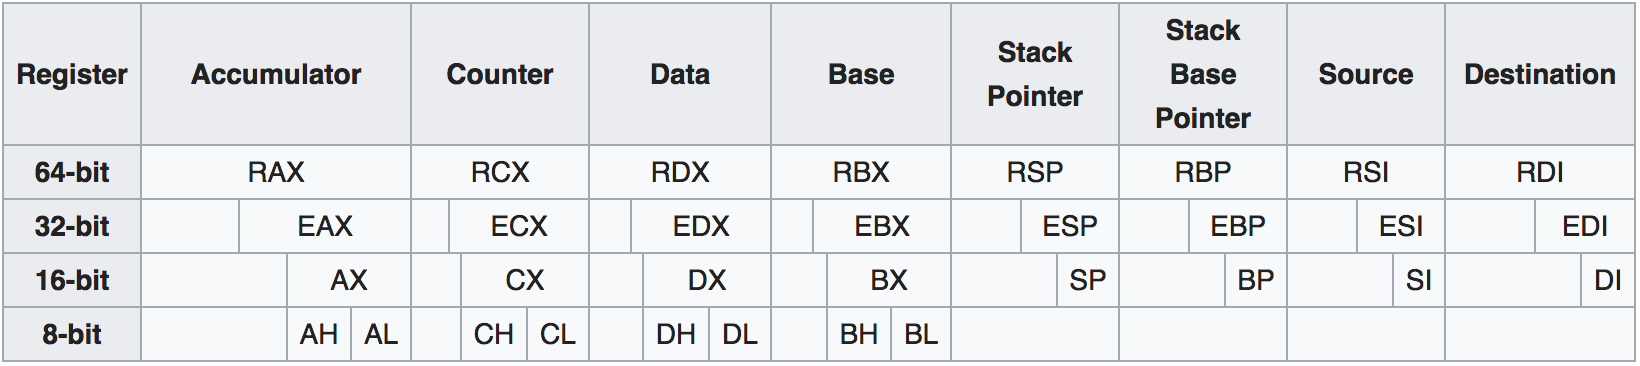
\includegraphics[width=.85\linewidth,keepaspectratio]{art/x86-regs.png}
	\caption{Usage of basic registers ordered by word size of the operating system on the x86 architecture.}
	\label{fig:x86-regs}
\end{figure}
The state (i.e value) of all the relevant CPU registers at a time $t$ is called a \textbf{context}. In VirtualBox, the CM keeps local copies of three of these contexts : a guest OS context, a special hypervisor context for the VMM and a raw context (a normal host OS context). When making a snapshot of the VM, the CPU Monitor actually saves the first two in order to subsequently put back the CPU exactly like it was at time $t$. Beside the saving aspect, holding three different contexts also allows VirtualBox to quickly switch between the guest and host "worlds" without the user noticing. This is very much necessary, because the whole point of the hypervisor is to make two different operating system coexist at the same time.

\hfill\textit{Relevant file }: \pathmono{src/VBox/VMM/VMMR3/CM.cpp}.

\subsection*{RAM Snapshot}

Another extremely important aspect of the state save is the dynamic memory aspect. How can VirtualBox completely separate the guest OS from the host without the guest noticing? This is done through the Page Manager (PM), a manager also taken into account by the Saved State Manager at snapshot time. 

\begin{wrapfigure}{l}{0.45\textwidth}
	\centering \scriptsize
	\vspace{-12pt}
	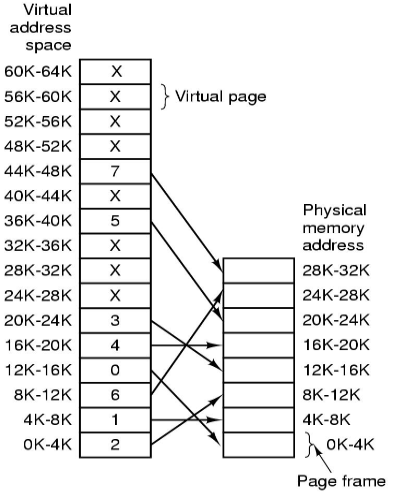
\includegraphics[width=0.40\textwidth,keepaspectratio]{art/mem-paging.png}
	\caption{Linux Mapping of Pages to Page Frames \cite{misc:mem-paging}}
	\label{fig:mem-paging}
	\vspace{-12pt}
\end{wrapfigure}
To better understand the Page Manager's job, we can look at a very similar concept : the memory paging technique used by the Linux operating system. As shown in \autoref{fig:mem-paging}, the way Linux abstracts the hardware from a running program is by offering said program an entire virtual address space as a sandbox. 

This virtual space is divided into fixed-length memory blocks (usually 4kB) called virtual pages that have a one-to-one correspondence to a random block of the same size in physical memory (page frame). Linux abstracts that correspondence with the help of a \gls{MMU} implemented in hardware, which translates virtual addresses into physical ones.

In the same way that Linux controls VirtualBox's physical memory accesses, the Page Manager controls the guest OS memory accesses. It enables the management of pages of memory allocated by the guest and adds one more level of memory indirection. For example, a program running on the guest OS will be executing operations on guest memory, but VirtualBox actually redirects them to operate directly on the physical address space offered by the host OS. This can be done with the help of two powerful concepts:
\begin{enumerate}
	\item \textbf{Binary translation}. This allows a software-assisted hypervisor like VirtualBox to "trap and virtualize the execution of sensitive, non-virtualizable instructions sets"\cite{online:virtualization}, like memory operations.
	\item \textbf{\gls{SLAT}}. Commonly known as \textbf{nested paging}, it allows a guest operating system to directly access the host's physical memory and thus removing a lot of overhead on memory operations.
\end{enumerate} 

Because the \gls{VMM} can hook to these memory operations in the guest OS, this makes the Page Manager aware of the page frames that belong to the guest OS. As a result, when a snapshot event occurs, the PM goes through its list of guest pages that were in use at that time and saves them. At restore time, this data is copied back someplace else in physical memory, and the translation table is updated accordingly.
 
\hfill\textit{Relevant file }: \pathmono{src/VBox/VMM/VMMR3/PGM.cpp}.
\section{Berkeley Lab Checkpoint/Restart for Linux}\label{sec:blcr}
As mentioned throughout this chapter, the problem of checkpointing a computer program can be solved at multiple levels depending on the needs. The approach that was taken by VirtualBox is very powerful, but it has major drawbacks:
\begin{enumerate}
	\item \textbf{Overhead processing}. The fact that an entire system gets simulated implies that virtualizing an operating system with a type-2 hypervisor like VirtualBox is basically an overhead cost on executing the program. 
	\item \textbf{Granularity}. It checkpoints the whole computer's state instead of one program. This is often too much granularity and can result in very large snapshot files. In the case of \gls{BBPSim}, this would be quite excessive.
	\item \textbf{Dependence on an hypervisor}. If the execution of the program had to happen inside an virtualized operating system, a simulation of the \gls{BBP} would have to rely on the use of an hypervisor. This not desirable, especially for the client.
\end{enumerate}

However, some other techniques can circumvent these limitations by taking by using a differing degree of checkpointing transparency, that is, at which abstraction layer the checkpoint takes place. Walters and Chaudhary define those layers as follows: 
\begin{shadedquotation}
\begin{enumerate}
	\item Hardware-level, additional hardware is incorporated into the processor to
save state.
	\item Kernel-level, the operating system is primarily responsible for checkpointing
running programs.
	\item User-level, a checkpointing library is linked into a program that will be responsible for checkpointing the program independent of the programmer.
	\item Application-level, the checkpointing code is inserted directly into the application by a programmer/preprocessor.
\end{enumerate}
\cite{paper:app-level-chkpt}
\end{shadedquotation}

\gls{BLCR} is one those attempts at creating a user-friendly method for checkpointing a Linux program. It is a program implemented at the Kernel-level, meaning that it is a module add-on to the Linux kernel and should be installed prior to running the user application.

\subsection*{Overview}
\gls{BLCR}'s solution is completely different from the one seen in \autoref{sec:virtualbox}, where checkpointing happens for every program running in the guest OS. It bases itself on the fact that properly controlling a program in a sandbox makes it checkpointable. This sandbox is provided by a kernel daemon, another process that runs in background in the kernel, that knows how to execute a checkpoint on a given program. 
\begin{figure}[htbp]
	\centering \small
	\includesvg[width=0.75\textwidth]{svg/blcr}
	\caption{Abstraction layers for an application sandboxed by BLCR.}
	\label{fig:layerblcr}
\end{figure}

There are several different ways to use \gls{BLCR}. An application-centric use case is shown in \autoref{fig:layerblcr}. To access the required utilities to checkpoint itself, the application code needs to have access to the library at compile-time. At runtime, the library (\pathmono{BLCR.so}) is then dynamically linked to the application code and the kernel-based BLCR process is put in charge of managing the application process' resources via the dynamic library. This management layer is necessary to properly save the application.

Checkpointing a program is done is done via shell commands to the background-running BLCR daemon:
\begin{tcolorbox}
\begin{minted}{bash}
cr_checkpoint --pid <PID>
\end{minted}
\end{tcolorbox}

where \texttt{PID} is the process ID of the checkpointable application. This command can be called programatically by the running application (via a \texttt{system()} call in the code), by another program or even by the user itself. Thus, checkpoints are sporadic in that context.

Once those commands are initiated, the \gls{BLCR} daemon outputs a context file containing the relevant information to restart back the application at this stage. At restore, the user must restart the application from the saved context file with another shell command:
\begin{tcolorbox}
\begin{minted}{bash}
cr_restart <path_to_context>
\end{minted}
\end{tcolorbox}
This fully restores the old application state: virtual address space, registers, thread and process IDs, file descriptors, signals. Basically everything not related to sockets or serial ports is put back the way it was.

%https://crd.lbl.gov/departments/computer-science/class/research/past-projects/BLCR/
%- see also virtualization technology : https://github.com/dmtcp/dmtcp (process-based)


\section{Checkpoint and Restore in User Space}\label{sec:criu}
https://github.com/checkpoint-restore/criu



%https://github.com/dmtcp/dmtcp


%super interesting : http://citeseerx.ist.psu.edu/viewdoc/download?doi=10.1.1.126.8121&rep=rep1&type=pdf
%https://www.usenix.org/legacy/publications/library/proceedings/usenix01/freenix01/full_papers/dieter/dieter_html/paper.html
}
%{
\setlength{\parindent}{2em}
\chapter{Methodology}\label{cha:meth}
Like any other project of its size, planning played an important part in this work's good completion. As the present thesis was made in the context of an internship at \gls{MDA}, its development had a lot to gain by adapting to the Dream Chaser team's development process. In addition, because the snapshot feature was a deliverable to the client (\gls{SNC}), it had to adhere as much as possible to certain guidelines, especially concerning deadlines and iterative feedback. Nonetheless, plenty of space was given for creativity and a methodology was adapted to work in parallel with the team. 

\section{Work on the DCCS}
First, the context had to be described, so that a methodology could be devised, both in the team development environment and the personal, more technical part.

\subsection*{Project Management}
The Dream Chaser team was composed mainly of four teams handling different aspects of the \gls{BBP}. There were two software and one FPGA teams, all of them overseen by the project management team. Most of the work as part of this thesis was done under one of the software teams, counting 10 members. And like many software teams choose to operate, the preferred development method was \textbf{Scrum}. 

Scrum is a very popular agile framework for all types of technical projects all around the world. It allows for a structured, well-defined development and delivery process for relatively small teams part of a complex product \cite{book:scrum}. The main goal of Scrum's usage in the Dream Chaser team was to effectively address its complex engineering problems while creating value for the product (the BBP and its embedded software) and adapting swiftly to unforeseen events during the project. A summary the important concepts of the development process is pictured in \autoref{fig:scrum-process}.

Following the framework's principles, the work of the software team was guided iteratively, using sprints. Their duration was set to two weeks from the start of the Dream Chaser project. This meant that every two weeks, the team took usually half a day to organize the next two weeks for each of its members. In particular, future collaborative work could be coordinated and work units ("stories") could be distributed from the backlog to the members during these "Sprint Review and Planning" meetings.

\begin{figure}[H]
	\centering
	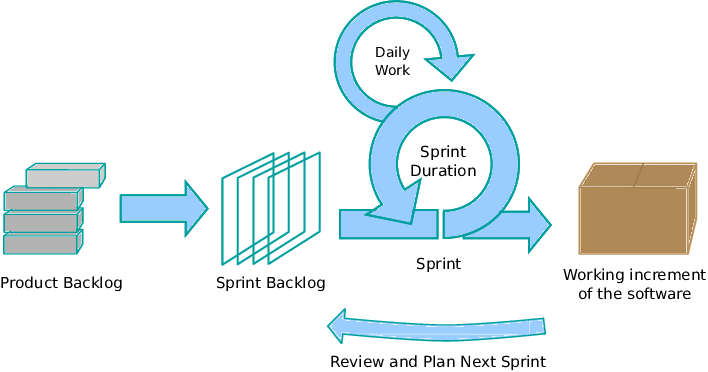
\includegraphics[width=0.9\linewidth,keepaspectratio]{art/scrum-process.png}
	\caption{The Traditional Scrum Life-cycle\cite{misc:scrum-process}}
	\label{fig:scrum-process}
\end{figure}

On top of these organization efforts, the team held 15-minutes meetings everyday, during which each member told the others what they had worked on in the past hours, raised up possible present or future blockers and mentioned the content of their pending work. These "dailies" allowed the team to stay productive, while quickly addressing any arising technical or organizational issues.

\subsection*{Integration of the Thesis Work in Scrum}
Of course, it was very important for this work to fit in the team's development scheme. After all, any project of comparable size needs a work structure and the fact that the team already had a well-working one meant it was an opportunity to adapt the academic project to a working-environment structure. Thus, this avenue was taken from the beginning of the thesis-internship.

Modifying the working method to make it \textit{scrum-able} turned out to have important benefits. For instance, rather than touching base only once in a while during the implementation phase, an update on the progress of the feature had to be given daily to the team. This way, they was able to get daily feedback on the progress of the save \& restore and could quickly provide support if needed. Such a situation happened on many occasions and a lot of time was saved by other members helping with rather technical questions or with finding relevant documentation. 

The dailies also brought the thesis subject "closer" to the team. Since the feature was linked to a customer requirement, it was critical for the team leader to have good insights on the overall progression and the predicted release date. A backlog of remaining stories linked to the feature had to be maintained for the team leader to be constantly up-to-date on the progression. Undoubtedly, knowing what to expect in the short and long term is always a big benefit for any project's organization. 

On top of everything, merging the thesis into the Scrum framework also allowed for a much better social integration and better working experience as a whole. 

\section{Breakdown into phases}
The save \& restore function in \gls{BBPSim} is a boolean feature: either it works and the simulator can consistently restart itself back to a previous state, or it doesn't. Like any other program, \gls{BBPSim} needs all of its components to function correctly. Therefore, partial saves of a simulation would lead to stability issues when restoring. 
In any case, such a binary feature should never be entirely programmed without incremental testing, because reverting back the strategy in the event of a failure would be too time-consuming.

This is why the thesis was broken down into phases, where each phase was considered done when it hit a certain milestone at the end. The milestones were chosen so that a save and a restore operation could be successfully done on one component or group of components in the simulator. In addition, in order to adapt the development of the feature to the Scrum framework, each phase was further divided into Scrum stories. That way, it was possible to estimate the time of completion of a certain milestone, since all stories in Scrum are subject to a time estimation before getting assigned. \autoref{tbl:project-phases} better shows how the thesis was divided. Since \gls{BBPSim} was a software with clearly defined layers, it was decided to fit the phases onto them.

This particular division was chosen, because most of the milestones also made the holding of demonstrations to stakeholders possible. Since this feature was part of a release of the simulator, \autoref{sec:feedback} further explains how the interaction with interested parties was handled.

\begin{table}[htbp]
	\centering
	\ra{1.2}
	\begin{tabularx}{\linewidth}{c X}
	\toprule
	\textbf{Phase} & \textbf{Milestone}\\
	\midrule
	1 & {Access to \gls{FSW} variables}\\
	2 & {Choice of state file format}\\
	3 & {Well-defined mechanism for restoring from file}\\
	4 & {\gls{DAS} memory layer saved \& restored}\\	
	5 & {Shared Memory layer saved \& restored}\\
	6 & {\gls{BBPSim} OS layer saved \& restored}\\
	7 & {\gls{BBPSim} Hardware layer saved \& restored}\\
	8 & {\gls{DAS} execution saved \& restored}\\
	\cmidrule{2-2} 
	-  & \textbf{Stable save \& restore}\\
	\cmidrule{2-2} 
	9 & {Snapshot of file system}\\
	10 & {Verification \& Validation integration}\\
	\cmidrule{2-2} 
	- & \textbf{Feature delivery}\\
	\bottomrule
	\end{tabularx}
	\caption{Division of the thesis work into phases and their milestone.}
	\label{tbl:project-phases}
\end{table}

\section{Customer and Internal Feedback}\label{sec:feedback}
As mentioned previously, this thesis was divided into phases, so that it would be possible to clearly keep track of the progress. However, the division was motivated by the ability to deliver periodic updates not only to the management team, but also to the customer.

As a contractor in the space sector, \gls{MDA} has everything to gain by having good commercial relationships with its customers. This is why meetings with \gls{SNC} were held during this project. Their main goal was to improve transparency with the client, but they were also used to gather important feedback to iterate over the feature's implementation details. 

As for internal feedback, sessions were also held every three to four weeks with members of the software and management teams. Their purpose was to demonstrate the evolution of the feature to stakeholders. As a side effect, this made the thesis "Proof-of-Concept-driven", because progress was motivated by getting the product demo-ready.
}
%{
\setlength{\parindent}{2em}
\chapter{Checkpointing Artifact} \label{cha:prod-artifact}
Before turning to the actual implementation of the save and restore feature, multiple choices of state representation needed to be considered. Whether one or more artifacts are produced for a checkpoint usually comes as a consequence of the approach that was taken in the design itself. However, in the context of this thesis, it was decided to start from the checkpoint artifact and build outwards. The save and restore feature was thus developed around that central idea.

\section{Design Constraints}\label{sec:file-constraints}
In sections \ref{sec:virtualbox} through \ref{sec:c3}, it was shown that the artifacts produced by checkpointing an application can take many forms. For instance, Checkpoint and Restore in User space outputs a series of files that each serve a different area of the restore, whereas VirtualBox produces one large file in a format defined as part of the open-source program. In the context of the BBP simulator, requirements DCMS-BBP-122 (see \autoref{tab:customer-reqs}) and U03 (see \autoref{tab:user-reqs}) forced the saving of a simulation to only output one file.

In addition, it was also important to take into consideration the amount of data that needed to be saved, as well as its nature. A preliminary investigation showed that the majority of the data was produced by the static variables inside the flight software (see \autoref{cha:das-impl}). It was also shown that the amount of data was of the order of 150MB. Since the weight of other software modules was considered negligible in comparison, this implied that most of the data contained within the state file had to be stored in binary.

It was also considered essential to be able to identify a checkpointing artifact from its content, not only by its name on the file system. Since the artifacts might be transferred frequently from one computer to another, especially inside a continuous integration system, forcing a naming convention on the file was not desirable.

Finally, even though a requirement concerning the number of artifacts was imposed, it didn't mention the usage of one format over another. For this reason, different alternatives were taken into consideration. 

\section{State File Format}
Since a lot of data had to be saved in the course of a simulation checkpoint, an appropriate file extension had to be determined. In the context of the save and restore feature design, it was important to evaluate the various file options. First of all, multiple potential candidates were researched. Then, each format was evaluated based on its general qualifiers and how well it performed in certain areas critical to the design, always bearing the constraints of \autoref{sec:file-constraints} in mind. To justify the decision quantitatively, a weighted rating in percent was performed. The assessment is shown in \autoref{tab:file-fmts}.

\begin{table}[htbp]
	\vspace{12pt}
	\centering
	\ra{1.3}
	\begin{tabularx}{\linewidth}{l c c c c c}
		\toprule
		&{\bfseries Readability}&{\bfseries Flexibility}&\makecell{\bfseries Library\\\bfseries Support}& \makecell{\bfseries Data-to-Size\\ \bfseries Ratio}&\multirow{3}{*}{\bfseries Total}\\
		\cmidrule{2-5}
		\multicolumn{1}{r}{\small Weight:}&{\small 5\%}&{\small 40\%}&{\small 15\%}&{\small 40\%}&\\
		\midrule
		Extended Markup Language  & 90 & 85 & 95 & 50& {\bfseries 72.75}\\
		YAML  & 80 & 80 & 75 & 75& {\bfseries 77.25}\\
		Binary  & 0 & 90 & 80 & 100& {\bfseries 88}\\
		JSON  & 80 & 85 & 80 & 65& {\bfseries 76}\\
		\bottomrule
	\end{tabularx}
	\caption{Evaluation of the relative strengths of multiple file formats as the output of a BBPSim checkpoint.}
	\label{tab:file-fmts}
\end{table}

The criteria used to assess of a format's performance are described as follows:
\begin{itemize}
	\item {\bfseries Readability}. How well can the format be read by a human? Is it possible to manually modify the file easily?
	\item {\bfseries Flexibility}. How customizable is the format with regard to data structure?
	\item {\bfseries Library Support}. Is there extensive, open-source support for this file format's generation?
	\item {\bfseries Data-to-Size Ratio}. What is the overhead of the serialization language? Does it scale well to hold binary data? Since the flight software contains variables that amount to around 100MB in total size, this criterion was weighted accordingly. 
\end{itemize}

Even though all the formats score reasonably well in flexibility and library support, some values from \autoref{tab:file-fmts} are still outsiders. For example, the binary format was given a score of 100 in data-to-size ratio, at the expense of readability. This is due to the nature of the format itself. With regard to data compressibility, there is no better than binary (assuming maximum theoretical data entropy\cite{art:shannon}). In the same category, for instance, it was found that XML needs to use the Base64 binary-to-text encoding to embed binary data, which can encode 6 bits of data into an \gls{ASCII} character that takes 8 bits\cite{art:base64}. This 33\% overhead is completely removed in the binary format. 

Binary also provides great flexibility, because it is up to the users to define a suitable format for their needs. There is no need to stay in the bounds of a defined structure like in the other data serialization languages.

With these reasons in mind, \ul{the binary format became the clear choice} as a state file output of a checkpoint in BBPSim.

\section{File Binary Interface}
Since a binary file presents great flexibility in how the data can be structured, this choice also required the development of a data serialization structure within the file, called a \gls{FBI}.

\subsection*{Record Blocks}
There are multiple ways of organizing data inside a binary file. The final arrangement is ultimately influenced by the needs of the developer and the application. In the context of this thesis, \autoref{sec:bbpsim-charact} established that a BBPSim simulation was composed of several modules that each operated inside a layer. When saving the state of the simulator, it was thus implicitly defined that the resulting file would need to package the modules' data such that it is easy to retrieve. To address this problem, the concept of \gls{RB} was developed. \autoref{tab:rb-fields} better explains each of the fields.

\begin{figure}[h]
	\vspace{6pt}
	\small
	\centering
	\includesvg[width=.8\linewidth]{svg/rb}
	\caption{Structure of a record block inside the checkpointing artifact.}
	\label{fig:rb}
\end{figure}

\begin{table}[h]
	\vspace{12pt}
	\centering
	\ra{1.3}
	\begin{tabularx}{\linewidth}{l c X}
		\toprule
		{\bfseries Name}&{\bfseries Size}&{\bfseries Description}\\
		\midrule
		Tag & 1 byte & Value that is associated to the content or type of data in the payload.\\
		\midrule
		Size & 4 bytes & The length of the payload in bytes. Expressed as an unsigned integer.\\
		\midrule
		Payload & {X byte(s)} & Raw bytes of data to save. Because of the Tag, this data can be correctly parsed, cast or loaded by the relevant simulation modules.\\
		\midrule
		CRC16 & 2 bytes & Calculation of the CRC16 error-detecting code on the payload section. This algorithms detects accidental corruption of raw data blocks.\\
		\bottomrule	
	\end{tabularx}
	\caption{Definition of the different sections that compose a record block.}
	\label{tab:rb-fields}
\end{table}

RBs are a binary construct that help segment and structure the state file. They were heavily inspired from the popular \gls{TLV} block format, used notably in the User Datagram Protocol definition\cite{report:udp}. To facilitate their manipulation programatically, it was decided that record blocks would be guaranteed to hold $\geq$1 byte of data in their payload. As for the decision of appending a \gls{CRC} calculation at the end of each RB, it was motivated by the certainty of holding valid raw data in the payload.

The payload section in each record block is not monitored by any mechanism. Hence, it is of the responsibility of the developer to correctly interpret the bytes of content. For instance, the users must ensure that the data endianness is correctly preserved when reading the file. Since the simulator runs exclusively on an machine with x86 architecture, little-endian can be assumed throughout the rest of this thesis.

\subsection*{File Layout}
Once the RB package format was defined, it was possible to design the general layout of the checkpointing artifact. Since \gls{BBPSim} was composed of various modules, and since each record block is parsable on its own (because of the embedded size), it was decided to simply queue them one after another. 

\begin{figure}[h]
	\vspace{6pt}
	\centering
	\small
	\includesvg[width=.8\linewidth]{svg/file-layout}
	\caption{Data layout of the checkpointing artifact.}
	\label{fig:file-layout}
\end{figure}

As shown in \autoref{fig:file-layout}, it was decided to prepend a file header to the list of record blocks. This was made with the intention of satisfying the constraint of file self-identification mentioned in \autoref{sec:file-constraints}. The information deemed necessary for identification of the checkpointing artifact was included in the header, described in \autoref{tab:header-fields}.
\begin{table}[h]
	\vspace{12pt}
	\centering
	\ra{1.3}
	\begin{tabularx}{\linewidth}{l c X}
		\toprule
		{\bfseries Name}&{\bfseries \Cpp Type}&{\bfseries Description}\\
		\midrule
		BBPSim Version & \texttt{char[20]} & String of the version of BBPSim that produced this artifact.\\
		\midrule
		FSW Version & \texttt{char[20]} & String of the version of the flight software that produced this artifact.\\
		\midrule
		Timestamp & \texttt{std::time_t} & When the artifact was created.\\
		\midrule
		Step Count & \texttt{uint32_t} & The number of times the \texttt{step()} command was called in the simulation that was saved.\\
		\midrule
		Load Address & \texttt{void*} & The address at which \pathmono{libBbpSim.so} was loaded.\\
		\midrule
		RBs & \texttt{uint16_t} & The amount of record blocks after the header.\\
		\midrule
		Reserved & \texttt{uint8_t[32]} & Reserved for future use.\\
		\bottomrule	
	\end{tabularx}
	\caption{Definition of the different fields in the state file header.}
	\label{tab:header-fields}
\end{table}

Since the save and restore can happen a long period of time apart, the BBPSim and flight software versions are necessary to identify whether a past checkpoint artifact is compatible with the current version. The timestamp and step counts were added for convenience. As for the addition of the load address of the BBPSim library, a detailed explanation is given in \autoref{cha:das-impl}. At the end of the header, some bytes were also reserved in order to keep the possibility of adding new fields without invalidating checkpointing artifacts produced in a previous version of BBPSim.

}
%{
\setlength{\parindent}{2em}
\chapter{Flight Software Checkpointing}\label{cha:das-impl}
At its core, offering a suitable environment for the simulation of the flight software was the main purpose of the BBPSim simulator. Since \gls{SNC} wanted to reproduce the in-flight behavior of the communication sub-system as faithfully as possible, the software-in-the-loop test framework was designed according to the principle of encapsulation: exclude all internal changes to the simulated software and instead build around what is already there. Having said that, inevitably, there were exceptions made for some parts of the flight software algorithms, where code had to be altered to make it compatible to run on a Linux machine. For the most part, however, as shown in \autoref{fig:bbpsim-layers}, BBPSim succeeded in integrating \gls{DAS} as an "untouchable" nucleus and interfacing only indirectly with it.

The fact that DAS was supposed to stay completely permeable to modification forced the implementation of the save \& restore feature to treat it as a black box. This point of view brought several challenges, which were not present when modifying the BBPSim code to support checkpointing. 

In this section, the constraints that influenced the development of a checkpointing technique within the flight software are first of all described. It should be noted that most of the solutions to the problems were based on technical details that, in the end, had a meaningful impact. Subsequently, \gls{DAS} is briefly analyzed to clearly define which of its components checkpointing was considered a necessary condition for a stable restore. Then, the approach taken to indirectly access, save and restore them is explained in details.

\section{Design Constraints}
It goes without saying that user and customer requirements played a big role in how the design went forward. In particular, to make the \gls{FSW} checkpointable, it was important to bear in mind DCMS-BBP-121 (64-bit application), U02 (no alteration to FSW) and U01 (no instability). However, some other technicalities had a big importance too. They are further detailed in this chapter.

Also, since the delivery method of BBPSim was through a Linux dynamic library, it was realized that most of the container-based solutions presented in \autoref{cha:state-of-the-art} could not apply to BBPSim. A shared object does not possess the same control as an application over many things, like memory layout. This was a problem, and a better explanation of the issue is given in the coming sections.

Finally, because the build process of the dynamic library happened inside a Linux machine, the tools used to execute the checkpointing had to be standard Linux programs installed on any distribution. This constraint came from the fact that developers on the Dream Chaser team used a Linux virtual machine to run simulations. Hence, adding the dependency on another program would imply changing all of the Linux VMs images on the team. This was of not desirable.

\section{Definition of Sufficient Condition for Restoration}\label{sec:conditions}
Saving and restoring an application was the main subject of \autoref{cha:state-of-the-art}. In most of the existing solutions that were presented, the checkpointer programs did not have any control over the building process of the checkpointee. This made them approach the checkpointing problem from various angles, depending on the level at which the program was supposed to interact with the checkpointed application. 

In parallel, they each introduced a different sufficient condition, in terms of what to save, to be able to restore back the checkpointee. For example, it was considered essential for CRIU to save the totality of active memory pages inside the application's \gls{VMA} range, something pointless using the C\textsuperscript{3} environment.

Since the checkpointing feature of BBPSim was done with a different set of constraints, the set of necessary conditions for a stable restore had to once again be revisited. In this section, an assessment of the required components to checkpoint in the flight software is done. 

\subsection*{Definition of FSW Program State}
The description of requirement DCMS-BBP-122 on page \pageref{tab:customer-reqs} mentioned that "the current state of the [BBPSim] model" had to be saveable between steps. Undoubtedly, the word "model" is a very abstract term, and it could be interpreted in many ways. It was important to first define what qualified as a "model" in the more concrete context of DAS.

To better picture this, a parallel can be drawn with how C code is structured once compiled. When the \gls{GCC} compiles a valid C source file on Linux, an object file with extension \texttt{.o} is produced. Internally, this file is laid out in the Unix-wide standard \gls{ELF}. This very flexible format is divided into multiple segments that each have their own function in defining the program at low-level.

In this context, there are four relevant memory segments inside an object file:
\begin{wrapfigure}{r}{0.45\textwidth}
	\centering 
	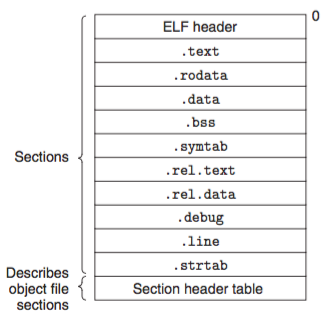
\includegraphics[width=.9\linewidth,keepaspectratio]{art/reloc-obj.png}
	\caption{Sections in an object file with ELF format.\cite{online:zhang}}
	\label{fig:sections-obj}
	\vspace{-24pt}
\end{wrapfigure}
\begin{enumerate}
	\item \textbf{\texttt{.bss}}. Contains the statically-allocated variables that were either left uninitialized or initialized to zero (in the source code).
	\item \textbf{\texttt{.data}}. Contains the statically-allocated variables that were initialized.
	\item \textbf{\texttt{.text}}. Contains the binary instructions. Basically, the executable code.
	\item \textbf{\texttt{.rodata}}. Contains the read-only data (constants).
\end{enumerate}
\autoref{code:c-to-segments} shows how the translation is done using real C code.

In this thesis, it is argued that the state, or "model" of the flight software could be defined by two main components: the memory segments of statically-allocated variables, and execution information. Taken in the context of an object file, the state of a multithreaded DAS can be explained as being:
\begin{shadedquotation}
The full contents of the \texttt{.bss} and \texttt{.data} segments for all FSW object files, the register set of each threads and the stack of each threads. 
\end{shadedquotation}

As for the \texttt{.rodata} and other segments, since they contain values that do not change from one simulation to the other, they were deemed unnecessary to include in this definition. The segments were identical at every simulation run, so it was superfluous to include them in the definition of the FSW state.

\subsection*{Condition 1 - Memory Segments}
The first necessary condition to be able to restore back to a previous "model" of DAS was to save the read-writeable, \textit{statically-allocated} regions in memory that concerned the flight software. It should be understood that a program's statically-allocated variables are variables that exist for the entire duration of the program. This term should not be confused with the \mintinline{c}|static| keyword of the C language, which limits the scope of a symbol in a compilation unit.

One can make an informal proof by contradiction of that statement by looking again at the sample code in \autoref{code:c-to-segments}. Let's suppose that, to restore DAS to a consistent global state, the restoration of the statically-allocated memory segments was not necessary. As a user, any changes done to variables (declared on lines \ref{lc-beg-statics} to \ref{lc-end-statics}) during a simulation would be lost, and therefore, the global state of the application would not be consistent with the one on the previous run. Variables on the second run would not read the same as they would have at the end of the first one. The inclusion of these segments is thus a necessary condition.

\subsection*{Condition 2 - Register Sets}
A second necessary condition for a consistent DAS global state restore was to save the register set of every thread attached to the DAS program. The \gls{PC} is located in this set, depicted in \autoref{fig:x86-regs}. It is the CPU register in charge of keeping track of which instructions are to be executed. Since CPU instructions are encoded in binary and reside in the same \gls{VMA} as the variables, they are also addressable. In that sense, the program counter register holds the address of the current instruction being executed by the processor. One can think of the PC as being "where" the thread is in its execution of the program.

In addition, it was also important to save the other general-purpose registers, which contained the context of the CPU at that particular moment. Not putting the correct value in the registers would produce a domino effect resulting in a segmentation fault at best, or undefined behavior at worst.

\subsection*{Condition 3 - Thread Execution Stacks}
Finally, saving the thread execution stacks was considered the last necessary condition to make the checkpointing feature work in the context of the flight software. An execution stack contains a lot of very important information about the thread. For instance, the function-local (scoped) variables are located in this stack. For reasons similar to the first condition, it was also important to save them.

On top of that, even though the program counter represents the position of the execution of a thread at a certain time $t$, the stack also contains its \textit{backtrace}, information about the "path" taken by the thread to get there. Precisely, the backtrace (or stack trace) is defined as the series of functions that were called consecutively until $t$. The stack-related concepts are treated thoroughly in \autoref{sec:das-exec-restore}.

\subsection*{Building the Sufficient Condition}
When the three conditions listed above were grouped together, it was defined that this formed a sufficient condition for a consistent DAS global state restore. More formally, this thesis argues that:
\begin{itemize}
	\item with $F$ being a C function in DAS;
	\item with $S_g$ being the global state of DAS memory in a first BBPSim run;
	\item with $S_s$ being the saved state restored in a second BBPSim run, defined as a subset of the global state in the first run ($S_s \subsetneq S_g$);
\end{itemize}
then
\begin{equation} \label{eq:sr_equiv}
	\forall F: F(S_s)\equiv F(S_g)
\end{equation}
when $F$ is void of non-deterministic processes. All DAS functions satisfied to this criteria, because they were strictly exempt of dynamic memory allocation, random numbers, and scheduling non-determinism (since the order of execution for threads was set at compile-time). An implication of the equivalence in \autoref{eq:sr_equiv} was that it was possible to observe the same behavior and output from a function in the simulated flight software if the required parts of memory were saved and copied back on the second run. It was not necessary to the save the whole contents of RAM ($S_g$), only a portion of it was necessary ($S_s$).

It should be noted that \autoref{eq:sr_equiv} also holds true whether $F$ is \textit{stateful} or stateless (i.e whether calling $F$ with the same parameters yields the same output or not). This is because even function-scoped static variables are included in the memory segments that are part of $S_r$. \autoref{code:c-to-segments} contains a good example of this. The \texttt{count()} function is stateful, but its state (i.e the value of \mintinline{c}|theCount|) is also included in the definition of the flight software state (in the \texttt{.bss} section).

Now that \textit{what} to save is properly defined, the following sections detail how the conditions were met for each of them to achieve a consistent checkpointing of the flight software.

%big sections
{
\setlength{\parindent}{2em}
\section{Black Box Symbol Access}\label{sec:das-mem-restore}
It was mentioned previously that, for integration reasons, the flight software code was considered unalterable (through requirement U02). Modifying the \gls{FSW} to accommodate the new checkpointing feature in BBPSim clearly defeated the purpose of encapsulation, and could potentially introduce errors in a critical piece of software. To represent reality as much as possible, the FSW was supposed to contain as fewer indications of the existence of \gls{BBPSim} as possible in its code.

In \autoref{sec:conditions}, it was shown that saving the entire set of statically-allocated variables in the DAS domain was a necessary condition for a stable restore. However, as it was forbidden to add \textit{getter} functions (e.g. \mintinline{c}|GetTheVariable()|) to access file-local variables from BBPSim, there needed to be a different solution. For the save and restore to be properly integrated, there needed to be a way to access them at runtime, a kind of indirect or "black box" access. 

In the end, the solution that was adopted involved the handling of DAS object files, \textit{after} they were compiled. Ultimately, no control over the flight software source code was given, but the compilation and building process were alterable. The following sections show how this limited control could be harvested, using a series of manipulations at build time, to give the \gls{BBPSim}-domain objects the required access to save the state of the flight software.

The whole process was quite complex, so one can get confused easily. For better visualization, the manipulations were drawn as a flowchart in \autoref{fig:blackbox-diagram}.

\subsection*{Linking Process}
First of all, it is crucial to understand how the linking process of an application is done. As mentioned earlier, when each source code file is compiled by \gls{GCC}, a \texttt{.o} object file is produced. Although this file contains executable code, the object file that would be produced by GCC would, by itself, not be enough to be executable as a stand-alone. The \textit{linker} needs to first process the object files. The one used in the case of this thesis was GNU \texttt{ld} version 2.27.

\begin{figure}[H]
	\centering 
	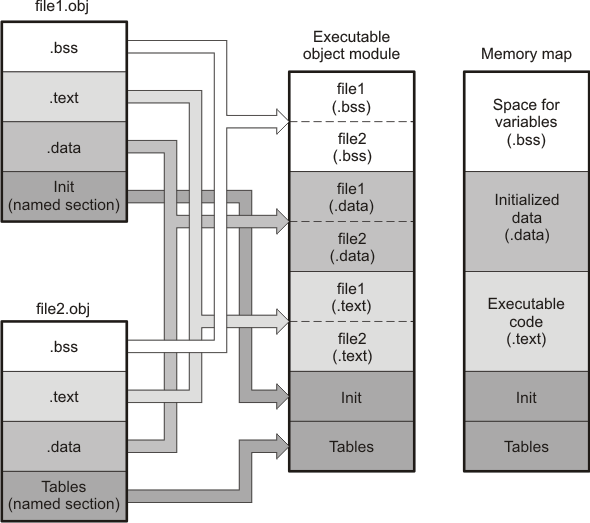
\includegraphics[width=.75\linewidth,keepaspectratio]{art/obj-to-elf-to-mem.png}
	\caption{Combining Input Sections to Form an Executable Object Module.\cite{online:linking}}
	\label{fig:link-mult-files}
\end{figure}

The linker's role in the building process is to combine each of the object files given as input into an executable file, or in the case of this thesis, a dynamic library. \autoref{fig:link-mult-files} better illustrates that concept. At linking time, \texttt{ld} groups the same segments from each \texttt{.o} file together and lays them sequentially in the executable object. Since object files can be given in an arbitrary order, the linker can make no guarantee on the final layout on its own.

In addition, while combining the object files together, the linker also resolves the undefined \textit{external} symbols, variables declared in one object file but used in another. 

Just like source code determines the resulting output of the compiler, it is also possible to control the linking process through the use of a linker script\cite{online:ld-scripts}. Even though, in most cases, users of the GNU linker don't provide a custom script, it is possible to specify one at linking time. 

Using such a script offers much more granularity to the developer in terms of which section gets put where in the executable object. In the field of embedded systems, this is particularly useful. Since components like non-volatile flash memory can be adressable by the CPU\cite{online:flash-ram}, it lets the developer decide whether certain sections should be written to flash (e.g. addressed from 0x10000 to 0x50000) or just be allocated in RAM before running the program.

\begin{listing}[H]
	\vspace{12pt}
	\begin{minted}{c}
SECTIONS
{
	. = 0x10000;
	.text : { *(.text) }//$\label{line:link-ex}$
	. = 0x8000000;
	.data : { *(.data) }
	.bss : { *(.bss) }
}
	\end{minted}
	\caption{Simple example of a GNU \texttt{ld} linker script.}
	\label{code:link-script-ex}
\end{listing}

One can read the example linker script in \autoref{code:link-script-ex}  sequentially. On line \ref{line:link-ex}, the script lays out the \texttt{.text} sections of all the object files sequentially inside the executable object's own \texttt{.text} section. This newly created section starts at address 0x10000 (represented by the "." keyword, the \textit{location counter}\cite{online:gnu-ld}). Then, the linker does the same thing for the \texttt{.data} and \texttt{.bss} sections, starting at address 0x8000000.

\subsection*{Clustering Flight Software Sections}
Since managing memory is always easier when it is contiguous, the first step that was taken to access the flight software memory was to group the sections of the relevant files together. This was done using a custom linker script. To make sure not to leave out any section, the default GNU \texttt{ld} linker script was used to make sure to start from a valid point. This script could be outputted from a shell with 
\begin{minted}{bash}
ld --verbose
\end{minted}
From that point, it was possible to partition the essential sections of the DAS object files only by changing the already valid script. These sections could be clustered in a special section of an intermediate shared object \pathmono{libBbpSim-intermediate.so}. 

As previously stated, one of the linker's job when building an executable is to resolve undefined symbols across all object files and to "interlink" them together. To do that, \texttt{ld} starts by looking in other object files to locate and set the correct addresses. Despite that, if said symbols are not defined in any object files, \textit{they can also be defined in the linker script}. This has two major implications: 
\begin{enumerate}
	\item Bi-directional transmission of values is possible (C code $\Longleftrightarrow$ linker).
	\item The source code can never know in advance the value of the undefined symbol if it's only defined during the linking phase.
\end{enumerate}

By harvesting these concepts together, two new contiguous sections of DAS variables in \pathmono{libBbpSim-intermediate.so} could be constructed. They are shown in \autoref{code:link-script-das}. For both the new \texttt{.das_state_vars_bss} and \texttt{.das_state_vars_data} sections, two symbols were defined as boundary variables to identify the start and end of the section in memory. A pair can be seen at lines \ref{line:bound-start} and \ref{line:bound-end}.

\begin{listing}[htbp]
	\vspace{12pt}
	\begin{minted}{c}
//...
.das_state_vars_data :
{
	__das_state_vars_data_start = .;//$\label{line:bound-start}$
	SORT(*obj/DasSrc/ *.o)(.data .data.* .gnu.linkonce.d.*)
	__das_state_vars_data_end = .;//$\label{line:bound-end}$
}
.das_state_vars_bss (NOLOAD) :
{
	__das_state_vars_bss_start = .;
	SORT(*obj/DasSrc/ *.o)(.bss .bss.* COMMON)
	__das_state_vars_bss_end = .;
}
//...
	\end{minted}
	\caption{Clustering of DAS variables via the \texttt{ld} linker script.}
	\label{code:link-script-das}
\end{listing}

It should also be noted that the \texttt{NOLOAD} parameter of the new \texttt{.das_state_vars_bss} section informed the linker that this memory section was to be zeroed out when the library was loaded, and thus not to allocate this memory inside the shared object itself. Otherwise, the library would be composed of nearly 100MB of zeros. And thanks to the inclusion of section guards, it was now possible to access the start and end addresses of the sections from C using:
\begin{minted}{c}
extern char __das_state_vars_data_start[];
extern char __das_state_vars_data_end[];
\end{minted}

To confirm that the script worked, an output map was produced by \texttt{ld} after the linking process (using \texttt{-Wl,-M=mapfile.map}). An excerpt is given in \autoref{map:ld}. It shows that the sections get created and that the \texttt{.data} and \texttt{.bss} sections of each DAS object file all get correctly mapped in the output file.

\subsection*{Cataloging State Variables}
Once the relevant sections of memory related to DAS were correctly laid out after the linking process, it was now a matter of deducing the address of each of these variables inside the resulting shared object. As the outputted file was in the ELF format, an ELF analyzing tool could then be used to get the list of all the variables contained within the relevant section:
\begin{minted}{bash}
objdump --syms -j .das_state_vars_data libBbpSim-intermediate.so
\end{minted}
Once the output was sanitized with \texttt{awk}, a big text file represented in  \autoref{das-symbol-catalog} was produced. This was called the \textit{symbol catalog}. One can observe various components in this file:
\begin{enumerate}
	\item The first line contains the SHA1 sum of the entire DAS source code repository. This was added to associate the list of variables to an existing source code for compatibility purposes.
	\item Each additional line represents a symbol that is contained in the flight software domain. They are laid out in the \verb|[<address> <size> <name>]| format. The addresses and the sizes are outputted in hexadecimal.
	\item The symbols defined as "guards" (\texttt{__das_state_vars_data_start}) earlier in the linker script were also included in this list. Because they don't represent any value in source code but instead hold an address, their size was zero.
\end{enumerate}

\subsection*{Including the Catalog in the Library}
Being able to generate a symbol catalog was very useful. However, there was a problem: with the way it was constructed, that catalog could never be included in the library. The catalog was generated from a finished shared object, but for it to ever be useful, the catalog needed to be accessible by the library at runtime. This created a chicken and egg problem, where both artifacts were dependent on one another.

The dependence was bypassed by transforming the symbol catalog into an object file and re-linking the library once again, including the new transformed catalog. 

Embedding raw bytes inside an executable file has been done since the early days of computing. For instance, it is possible for a malicious programmer to embed executable code within a self-extracting archive file\cite{online:sfx}. In the case of BBPSim, which was an ELF running on an x86 64-bit machine, it was possible to embed the catalog, as a string, \textit{inside} the library itself by first transforming it into a \texttt{.o} file:
\begin{minted}{bash}
objcopy --input binary --output elf64-x86-64          \
--binary-architecture i386:x86-64                     \
--rename-section .data=.das_state_vars_catalog_string \
das-symbol-catalog.txt                                
\end{minted}

This put the raw bytes of the catalog in the \texttt{.das_state_vars_catalog_string} section of the \pathmono{das-symbol-catalog.o} file.

The second part consisted in correctly laying out those bytes in the second and final shared object, \pathmono{libBbpSim.so}. This was done by once again taking advantage of the linker script in \autoref{code:link-script-das} to add an additional section, \texttt{.das_state_vars_catalog_string}.

Finally, all the object files both from the BBPSim and DAS domains could be linked a second time, together with \pathmono{das-symbol-catalog.o}. The resulting \pathmono{libBbpSim.so} file would be the last and final shared object. This effectively embedded the symbol catalog's raw bytes, encoded in \gls{ASCII} characters. Executable code inside the library could also refer to the stringized symbol catalog via newly created symbols used as guards for the raw bytes. Those symbols being only defined in the second linking process, it was necessary to tag them as having \texttt{weak} linkage for the linker not to complain on the first linker pass:
\begin{minted}{c}
extern char __attribute__((weak)) _binary_das_symbol_catalog_txt_start[];
extern char __attribute__((weak)) _binary_das_symbol_catalog_txt_end[];
\end{minted}

The results can be better shown by using a binary visualization program\cite{online:binvisio}. \autoref{fig:bin-lib-comp} shows a comparison of the \pathmono{libBbpSim-intermediate.so} and \pathmono{libBbpSim.so} shared objects in binary. Bytes with a value in the \gls{ASCII} character range are represented in blue. Both images read left-to-right with address 0x0 on the left. It is possible to see that a new blue section appear in \autoref{fig:bin-lib-final}, thus confirming that the symbol catalog correctly got included in the final version of the BBPSim library.

\begin{figure}[htbp]
	\centering
	\begin{subfigure}{\linewidth}
		\centering
		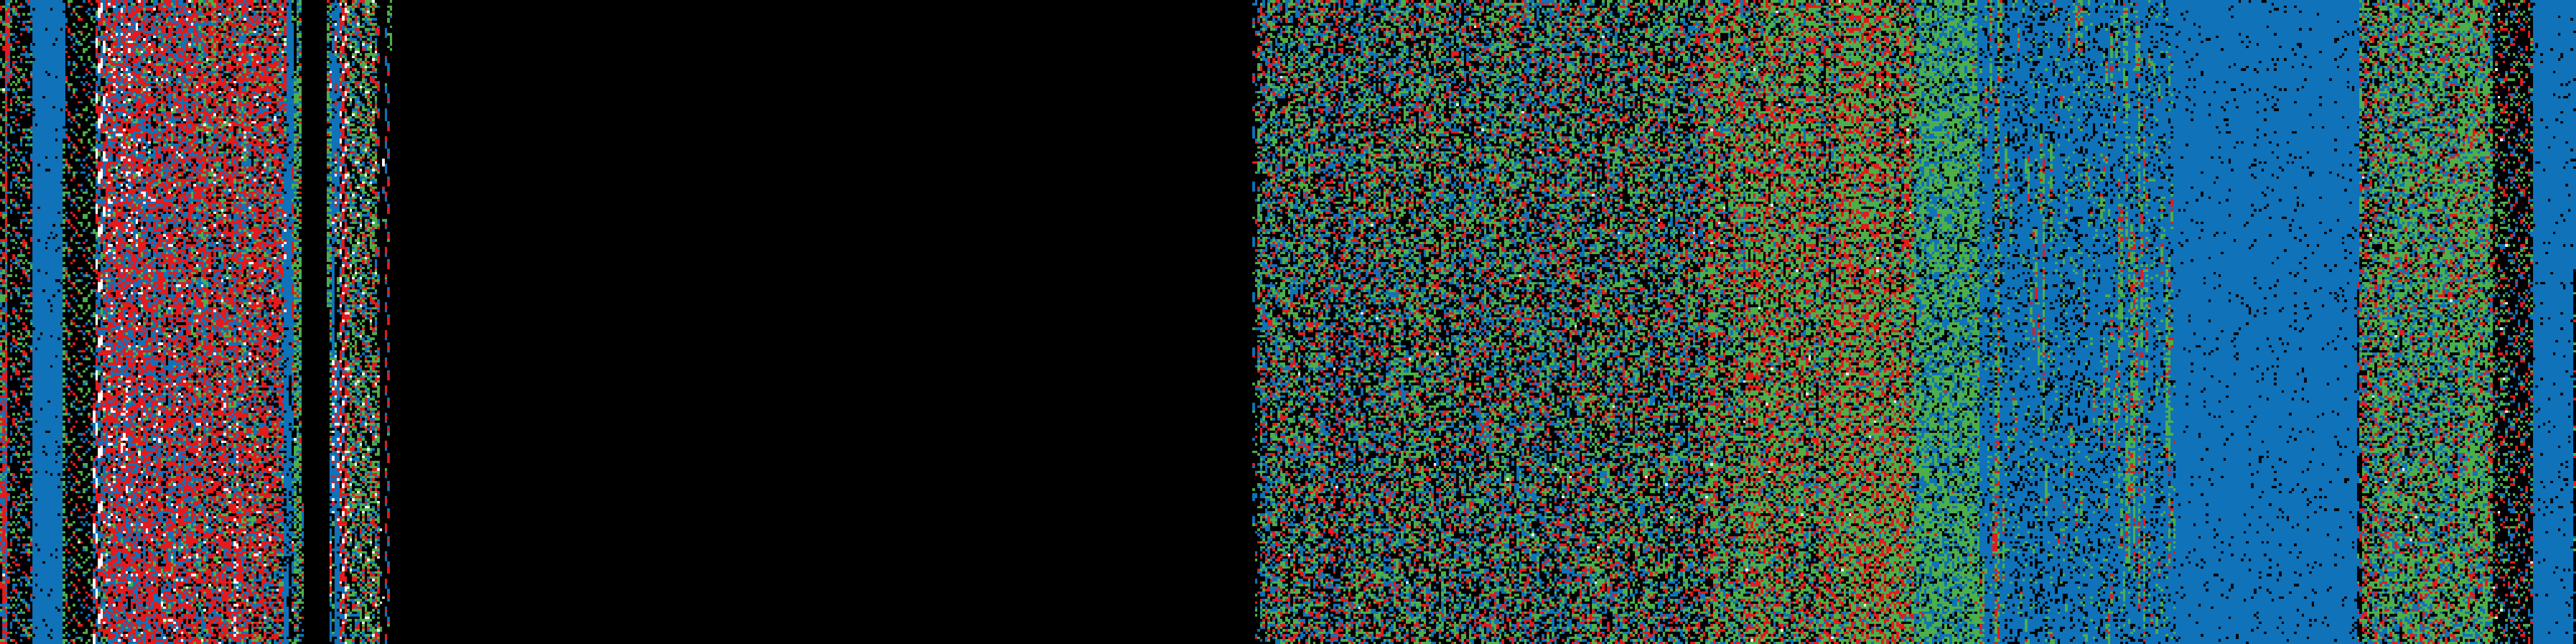
\includegraphics[width=\linewidth, keepaspectratio]{art/bin-lib-intermediate.png}
		\caption{Binary visualization of \pathmono{libBbpSim-intermediate.so}}
		\label{fig:bin-lib-intermediate}
	\end{subfigure}
	\vspace{12pt}
	\begin{subfigure}{\linewidth}
		\centering
		\includegraphics[width=\linewidth]{art/bin-lib-final.png}
		\caption{Binary visualization of \pathmono{libBbpSim.so}}
		\label{fig:bin-lib-final}
	\end{subfigure}
	\caption{Comparison of the resulting libraries after the first and second linking process.}
	\label{fig:bin-lib-comp}
\end{figure}

Since there was no modification to the DAS object files between the two linking process, the variable list taken from \pathmono{libBbpSim-intermediate.so} \textit{was guaranteed} to be the same and in the same order as \pathmono{libBbpSim.so}. This embedding of data also did not violate the ELF specification, which is clear about it's requirements:

\begin{shadedquotation}
[...] sections and segments have no specified order. Only the ELF header has a fixed position in the file.\cite{online:elf-spec}
\end{shadedquotation}

\subsection*{Shared Object Considerations}
As stated previously, the delivery method of BBPSim was done through a shared object, or dynamic library. This brought some challenges pertaining to memory validity, since the behavior of those objects is very particular.

When a program links a shared library, it is the job of the \textit{dynamic linker} to load that library in the program's address space at runtime. This special tool performs many things, from load-time relocation to symbol references resolving\cite{online:elf-reloc}, which are all done before the \texttt{main()} of the program is called. In particular, the dynamic linker starts by mapping the different sections of the dynamic library inside the address space of the program. 

\begin{figure}[htbp]
	\centering
	\begin{subfigure}[t]{.58\linewidth}
		\small
		\centering
		\includesvg[width=\linewidth]{svg/ptr-mem-first-run}
		\caption{Contents on the first run.}
		\label{fig:ptr-mem-first-run}
	\end{subfigure}%
	\begin{subfigure}[t]{.38\linewidth}
		\small
		\centering
		\includesvg[width=\linewidth]{svg/ptr-mem-second-run}
		\caption{Contents on the second run}
		\label{fig:ptr-mem-second-run}
	\end{subfigure}
	\caption{Potential displacement of pointed object with ASLR enabled.}
	\label{fig:mem-displacement}
\end{figure}

In Linux, the concept of \gls{ASLR} tells the dynamic linker to randomize the location at which the shared library's sections are loaded with every program run. A problem arose with the use of pointers in flight software: because of ASLR at restore time, pointer variables would become invalid, since what they pointed would not be located at the same address, like in  \autoref{fig:ptr-mem-second-run}. This problem did not have a straightforward solution. For this reason, \gls{SNC} was asked if disabling \gls{ASLR} on their Linux machine would be reasonable, and the request was accepted. This meant that \pathmono{libBbpSim.so} would always be loaded at the same address, hence avoiding this problem. The address was one of the fields in the checkpointing artifact header (see \autoref{tab:header-fields}).

\subsection*{Summary}
This method of indirect access to DAS variables efficiently served its purpose. It defined a way for the BBPSim domain objects to access flight software memory without requiring the modification of software, since everything happened at build time. It deduced the address of the variables rather than depending on an API like \texttt{GetTheVariable()}. This fulfilled the first necessary condition for a stable restore, defined in \autoref{sec:conditions}. One of the big benefits of this approach was that potential addition of new variables to the flight software would be automatically taken in charge, thus the solution was future-proof.

In \autoref{cha:bbpsim-impl}, how the catalog was used by \gls{BBPSim} is further described.
}
\section{FSW Execution Backup and Restore}\label{sec:das-exec-restore}
In \autoref{sec:bbpsim-charact}, the most important characteristics of the BBPSim environment were discussed. In particular, it was seen that the flight software was a multithreaded application running inside the \gls{BBPSim} environment. Because simulations had to run on a Linux machine, the threading API had to be re-implemented by BBPSim to be built on top of the POSIX threads library (\textit{pthread}), which is extensively supported by Linux. 

Saving the execution "point" of each thread was an important part of the design of the checkpointing feature in BBPSim. At restore time, it was vital to put back the threads execution to the point they were before in the code. However, playing with threads was not trivial, since they are an entity that is completely abstracted in C code.

In this section, some approaches that attempted to resolve the execution restore problem are first of all described, along with why they didn't work or couldn't apply in the case of BBPSim. Then, a description of the checkpointing, saving and restoring operations that were adopted in this thesis is given, together with how they fulfill the last two necessary conditions to a stable flight software restore, given in \autoref{sec:conditions}. 

\subsection*{Possible Solutions}
For simplicity reasons, it is often more useful to reduce the complexity of the problem and then scale up the solution to apply it in the real case. For this thesis, the single-threaded restore had to first be solved before attacking the multithreaded aspect. 

While in a simulation, when it is in standby between two step commands, a flight software thread could hold one of three possible states:
\begin{itemize}
	\item \textbf{Fresh}. The thread was created (using the Deos API function \texttt{createThread()}) at the previous step but never actually given CPU time to execute. The thread is pending on a signal (a semaphore).
	\item \textbf{Mature}. The thread has executed for at least one step. This implies that it has called \texttt{waitUntilNextPeriod()} at least once.
	\item \textbf{Dead}. The thread was terminated at the last step, either by itself or another running thread.
\end{itemize}

Three different strategies were attempted to solve the execution restoring problem. One can take \autoref{code:example-task} as an example of a flight task loop to follow through.
\begin{enumerate}
	\item \textbf{Restart back fresh and mature threads from scratch}. This had obvious problems.  Cold-starting all the threads alive when restoring would mean the task preamble (everything \textit{before} the infinite loop) would get executed twice: once at the first simulation and a second time when restoring. Since embedded utilities like mutexes also got restored, the flight software would try to re-create them when restoring. This would inevitably create runtime errors.
	
	\item \textbf{"Replay" the mature threads until their first \texttt{waitUntilNextPeriod()}}. This implied that the \texttt{create*()} Deos API functions had to somehow be skipped, such that no embedded utility was created. The thread would then be replayed until its \texttt{waitUntilNextPeriod()}.
	
	Since \gls{BBPSim} was an \gls{ELF} dynamic library, this option consisted in hooking on these API calls, and redirecting them to stub functions that did nothing. The strategy was possible by using a complex set of operations that overwrote addresses in the look-up table used to resolve dynamic library function addresses, the \texttt{.rel.plt} section.\cite{online:shoumikhin}.
	
	This would have been a good solution, if only for the fact that tasks could contain more than one \texttt{waitUntilNextPeriod()}. There was nothing prohibiting a task to call \texttt{waitUntilNextPeriod()} in its preamble, for example. There was actually many occurrences of this in the flight software, for instance when threads wait for messages from other threads before starting their own task loop.
	
	With this in mind, it was necessary to find out \textit{at which} instance of \texttt{waitUntilNextPeriod()} the thread was saved, and when exactly should the Deos API be "re-enabled". This was considered as a poor approach with too many corner cases to be implemented effectively.
	
	\item \textbf{Reconstruct the entire threads}. This was the candidate kept for this thesis. Choosing this solution implied that everything required to reconstruct the thread needed to be included in the checkpointing artifact, hence the last two necessary conditions of \autoref{sec:conditions}. 
	
	The process relied on two facts: 1. \pathmono{libBbpSim.so} was always loaded at the same address no matter the simulation, and 2. both saved and restored simulations were ran on the same x86-64 machine. 
\end{enumerate}

In the previous sections, it was seen that, to restore back a simulation to its previous state, one had to backup two components pertaining to flight software execution: one set of CPU registers per thread and one execution stack per thread. In the following sections, the strategy used to gather these components is further detailed.

\subsection*{Checkpointing the CPU Register Set}
The first step in saving a thread's execution state was to come up with a way to make the flight software code checkpoint itself. In particular, it was important to obtain a set of registers associated with that thread at the end of every simulation step.

Saving such a register set was absolutely necessary to restore the flight threads without stability issues. The registers contained important information about what the thread was doing. In particular, this set contained the \textit{program counter}, pictured in \autoref{fig:x86-regs}, which itself held the address of the machine instruction the thread would be currently executing. The register set also contained the stack pointer, which pointed on top of the thread's execution stack.

For obvious reasons, it was vital to save this register set \textit{at the right time} in the execution. If the registers were snapshotted at the wrong moment, the program counter would not be pointing to a viable instruction, which would make the restore operation crash. This problem was highlighted by the thread scheduling technique implemented by BBPSim. In \autoref{fig:step-cmd}, it was shown that flight software threads were executed one after another at every simulation step. In practice, this mechanism was implemented with two semaphores. Each thread was pending on a "go" semaphore inside BBPSim's \texttt{waitUntilNextPeriod()} reimplementation. Once the scheduler signaled the semaphore, the thread executed a task loop until it returned inside the \texttt{waitUntilNextPeriod()} function, which signaled back to the scheduler that the thread was done. This procedure is shown in \autoref{code:thr-sched-bbpsim}.

\begin{listing}[htpb]
	\centering
	\begin{minipage}{.5\textwidth}
	\begin{minted}{c}
void Task() {
	//task premable here
	
	while(true) {
		//task loop content here
		waitUntilNextPeriod();
	}
}
	\end{minted}
	\end{minipage}%
	\begin{minipage}{.5\textwidth}
	\begin{minted}{c}
//re-implementation of Deos API
void waitUntilNextPeriod() {
	//loop finished, signal returned
	sem_post(&return_sem);
	//wait for go from scheduler 
	sem_wait(&go_sem);
}
	\end{minted}
	\end{minipage}
	\caption{Thread scheduling procedure in BBPSim.}
	\label{code:thr-sched-bbpsim}
\end{listing}

If the register snapshot happened after a simulation step (using \mintinline{c}|ptrace()| like \gls{CRIU} in \autoref{sec:criu}), all the threads would be waiting inside the \mintinline{c}{sem_wait()} function, which relied on a semaphore artifact that would not be valid anymore at restore time. Therefore, another approach was needed.

The solution chosen for this problem needed the thread to checkpoint \textit{itself}, in order to gather its own set of registers from within its own domain (i.e. inside DAS code). Requirement U02 did however forbade any modification to the flight software. Consequently, the injection of checkpointing code within the flight software was taken as the main strategy. By redefining the \texttt{waitUntilNextPeriod()} symbol, it was possible to inject code that would save the registers at the right moment. This could be done by using the compiler's preprocessor to convert source code before actually compiling the code, like in \autoref{code:chkpt-inject}. By harnessing the GNU C library's types and functions for user-implemented context switching\cite{online:getcontext}, this injection would transform the flight software at compilation to checkpoint itself at the end of every loop, before calling the real \texttt{waitUntilNextPeriod()}. 
\begin{listing}[htpb]
	\centering
	\begin{minted}{c}
#define waitUntilNextPeriod()                         \
do                                                    \
{                                                     \
	ucontext_t* chkpt = GetThreadCheckpointSaveSlot();\
	getcontext(chkpt);                                \
	waitUntilNextPeriodReal();                        \ 
} while(0)

void waitUntilNextPeriodReal() //<- redefined
{
	//semaphore signaling here
}
	\end{minted}
	\caption{Injection of checkpointing code in the flight software.}
	\label{code:chkpt-inject}
\end{listing}

This had big benefits, because register snapshots (done with \mintinline{c}|getcontext()|) would be done inside flight software code, and would thus enable BBPSim to restart back the execution inside the task loop directly. The restored thread would then run until it called \texttt{waitUntilNextPeriodReal()} to wait for the scheduler's "go" signal.

Because the \gls{BBPSim} library would always be loaded at the same address, the program counter that would get saved at this stage would still be valid at restore time. It didn't matter if this was the first simulation or a second restored simulation, the PC would remain valid in-between because it would be pointing to the same instruction. 

This effectively satisfied the second necessary condition for a stable restore, defined in \autoref{sec:conditions}, which was to save the register set of all threads.

\subsection*{Execution Stack Layout}
Properly understanding how the reconstruction of threads was accomplished requires one to first grasp basic execution stack operations principles. As the target machine was based on the x86-64 architecture, this thesis focuses on call stacks produced by this architecture, although the concepts might very well be applicable to others.

The execution stack (also called \textit{call stack}) is a data structure that holds information about the series of functions that were called up to present time. There is one stack per thread of execution in a given program. The stack is a low-level object that keeps track, for every caller function, of the point where the execution should be resumed after the callee returns. This is done through the use of stack frames, which represent calls to subroutines that haven't yet returned. The general layout of this structure in memory is pictured in \autoref{fig:call-stack-layout}, where a caller (\texttt{DrawSquare}) calls a callee (\texttt{DrawLine}). In the x86 architecture, the stack is downward-growing (i.e. from high address to low).

\begin{figure}[htbp]
	\centering
	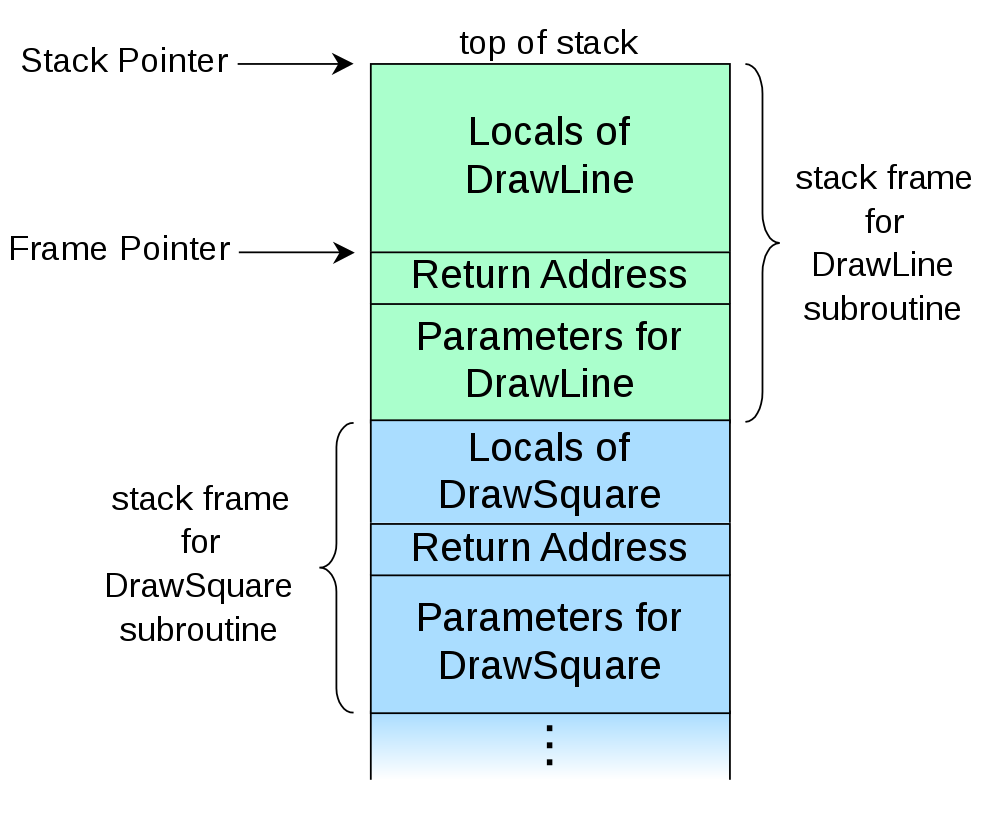
\includegraphics[width=.6\linewidth,keepaspectratio]{art/call-stack-layout.png}
	\caption{Call stack layout for downward-growing stacks\cite{online:stack-img}}
	\label{fig:call-stack-layout}
\end{figure}

The image also shows other important items for proper call stack operations. The \textit{stack pointer} (also in \autoref{fig:x86-regs}) is a CPU register that always points to the top of the stack, at the last accessible address. Another notable CPU register is the \textit{frame pointer}, or base pointer (\texttt{rbp}), which points at the base of the currently active stack frame. 

\subsection*{Accessing Thread Execution Stacks}
When using the usual \mintinline{c}|pthread_create()| API function, one simply has to provide a function as a parameter to create a new thread. Using the default parameters, this call makes the operating system allocate memory for the thread's stack, and then schedules it\cite{online:pthread-create}.

It is however possible for users of the POSIX threads library to specify a region of memory to use as stack space by specifying the attributes with \mintinline{c}|pthread_attr_setstack()|. This simple solution for thread stack execution access by BBPSim was thus chosen. Before starting any flight software thread, \gls{BBPSim} was modified to allocate 2MB of memory for it, which was considered to be sufficient for this application. It should be noted that this block of memory was required to be page-aligned to a virtual memory page. As a result, BBPSim held a reference to every thread's stack. It was then possible to include them in the checkpointing artifact, hence satisfying the third and last necessary condition for a stable restore.

\subsection*{Reconstructing Flight Software Threads}
Once the necessary components were saved as part of the first BBPSim simulation, both the fresh and mature threads had to be brought back in the same state as they were before. Nevertheless, the past execution stacks and register sets weren't enough, by themselves, to be able to restart the past threads. Some meticulous manipulations of that data had first to be done. 

Indeed, the reconstruction of flight software threads had to reconcile two different ecosystem together. From the operating system's point of view, the threads that were spawned in the second simulation run were completely different from those on the first. But from the flight software's perspective, the threads had to be, functionally speaking, the same. In that sense, one couldn't simply copy the old stack onto the new and expect the thread's execution to continue seamlessly. One reason for this is that important scheduling information was contained at the base of the stack, at higher addresses. 

To solve the problem, this thesis presents a way to reconstruct the old flight software threads by using new threads and meticulously replacing their stack frames with old frames. 

First of all, it was important to define the concept of \textit{user stack}. The stack of a pthread was divided in four main spaces, like \autoref{fig:stack-spaces} shows. The first two spaces were defined as containing all call frames pertaining to functions in the C and pthread libraries respectively, which use low-level Linux routines to coordinate the creation of the thread. As for the user stack space, it was defined as being the portion that contains all the frames related to \textit{user-defined functions}. In that sense, the \textit{user stack start} was defined as being located at the first 64-bit-aligned address after the pthread stack space. 
\begin{figure}[htbp]
	\centering 
	\includesvg[width=.8\textwidth]{svg/stack-spaces}
	\caption{Division of the execution stack into spaces.}
	\label{fig:stack-spaces}
\end{figure}

Because C code abstracts low-level constructs, finding the beginning of the user stack required the use of assembly. This was done by using \gls{GCC}'s inline assembly tools at the beginning of the first user function (the one provided to \mintinline{c}|pthread_create()|), as \autoref{code:usr-stk-start} shows\cite{online:inline-asm}. Once this address could be accessed, it was possible to deduce the total user stack start offset in any stack $s$ by subtracting the stack top's address:
\[
	\Delta_{usr}=s_{usr}-s_{top}
\]
Once this offset was obtained, it was crucial to include it in the checkpointing artifact, since pthreads don't necessarily \textit{always} have the same $\Delta_{usr}$. 
\begin{listing}[htpb]
	\centering
	\begin{minted}{c}
void bbpsimThreadEntry() {
	uint64_t x[4]; //0x20 bytes 
	asm volatile("mov %%rsp, %0  \n\t" //get current stack pointer
                 "addq $0x20, %0 \n\t" 
                 : "=r" (fswthread->m_pi8StartUserStack) //=$s_{usr}$
                 :);
	flightSoftwareTask(); //<- call never returns
}
	\end{minted}
	\caption{Capture of the user stack start.}
	\label{code:usr-stk-start}
\end{listing}

From then, it was possible to reconstruct the thread's execution stack the way it was before by copying only the user and unused portions of the old stack onto the new. This operation was done by the thread itself, using another inline assembly routine located in the restoring function. This stack-copying operation had to be done meticulously. It was important not to "pollute" the resulting stack, and thus this is why assembly was once again the perfect candidate. The ability to handle the registers manually could provide the required granular control. The complete thread reconstruction routine is included in \autoref{code:stk-copy-asm}. In the code, it is possible to observe many things. First, the \texttt{copyquadword} subroutine (at line \ref{code:copyqword-beg}) is called many times in order to copy the old user stack on the new one, starting from the correct offset. Then the routine jumps to \texttt{setcontext()}, which overwrites the current register set with the old one. This call should never return, because it sets the program counter to point back into the flight software code. Because \texttt{setcontext()} itself makes use of the stack\cite{online:setcontext}, it was important to first make the stack pointer point at an appropriate address, so as to not pollute the stack portions that were just written to. In the end, making a live thread replace its own stack frames could qualify as a careful stack corruption exercise, which is pictured in \autoref{fig:stack-reconstruction}.

\begin{figure}[htbp]
	\centering
	\begin{subfigure}{.33\linewidth}
		\centering\small
		\includesvg[height=\linewidth]{svg/stack-reconstruction1}
		\caption{Restored thread before}
	\end{subfigure}%
	\begin{subfigure}{.33\linewidth}
		\centering\small
		\includesvg[height=\linewidth]{svg/stack-reconstruction2}
		\caption{Old frames overwritten}
	\end{subfigure}%
	\begin{subfigure}{.33\linewidth}
		\centering\small
		\includesvg[height=\linewidth]{svg/stack-reconstruction3}
		\caption{Copy of the old frames}
	\end{subfigure}
	\caption{Stack reconstruction process.}
	\label{fig:stack-reconstruction}
\end{figure}

Keeping in mind that the \gls{BBPSim} library was always loaded at the same address, replacing the entirety of the new user stack by the old one had big benefits:
\begin{itemize}
	\item \textbf{Backtrace information was preserved}. This meant that, when using GDB to debug a restored simulation, the debugger would correctly find the return addresses in each stack frame (see \autoref{fig:call-stack-layout}) and could thus display the exact call stack that was just restored. The approach "fooled" GDB into thinking this new stack was there all along.
	\item \textbf{Stack variables were preserved}. With the way everything was copied over, even variables allocated on the stack would hold the same value. This meant that function-scoped variables could hold the same value as before.
\end{itemize}

Using this low-level approach, the restoring of a thread was near instantaneous, fulfilling customer requirement DCMS-BBP-56. The only cost was the stack-copying subroutine, which couldn't really be more optimized than the one in \autoref{code:stk-copy-asm}.

\subsection*{Solution Limitations}
Of course, using such a technique brought its lot of drawbacks. Since the old stack was copied integrally, this meant that stack-allocated pointers were put back as well, and thus held the same value as during the first simulation. In flight software, this was mitigated mainly for three reasons: 
\begin{enumerate}
	\item The address of static DAS variables was always the same, so those pointers would point to a valid address.
	\item Dynamic memory allocation wasn't used, so addresses were deterministic. BBPSim objects, though, were allocated dynamically, and some BBPSim-defined Deos types had to be modified to address the issue. This subject is treated in \autoref{cha:bbpsim-impl}. 
	\item The amount of old stack frames to copy back was low. This is because end-of-task-loop calls to \texttt{waitUntilNextPeriod()}, which checkpointed the flight software, were nearly always located in the task loop (i.e. when in the first user stack frame). This characteristic mitigated problems related to using the address of a function-local variable as a pointer parameter to another function, which would have been invalidated by the restoring process. 
\end{enumerate}

This process was also limited in the fact that the \texttt{-fomit-frame-pointer} GCC option unconditionally needed to be enabled. As the x86 architecture states, the frame pointer of the caller is usually pushed on the stack when calling a function\cite{online:x86-abi}. This means that the stack usually contains data that points inside \textit{itself}. As thread stacks were dynamically allocated, and thus were never located at the same place in memory, frame pointers were a big problem. Adding the GCC option when compiling every C and \Cpp file completely removed that limitation by taking out the reliance on the frame pointer entirely. It results in slight modifications to the compiled program, which changes the access to stack-allocated variables to be based on an offset from the \textit{stack pointer} rather than the frame pointer\cite{online:omit-frame-pointer}.

Finally, this solution was definitely not portable. Although this wasn't a problem for BBPSim, using the presented technique to cover a wide range of architecture in a general program would not work without extensively rethinking it. In addition, the use of inline assembly is compiler-specific. Even though GCC is very popular, this stack-copying approach is still locked to this compiler. 



}
\section{FSW Execution Backup and Restore}\label{sec:das-exec-restore}
In \autoref{sec:bbpsim-charact}, the most important characteristics of the BBPSim environment were discussed. In particular, it was seen that the flight software was a multithreaded application running inside the \gls{BBPSim} environment. Because simulations had to run on a Linux machine, the threading API had to be re-implemented by BBPSim to be built on top of the POSIX threads library (\textit{pthread}), which is extensively supported by Linux. 

Saving the execution "point" of each thread was an important part of the design of the checkpointing feature in BBPSim. At restore time, it was vital to put back the threads execution to the point they were before in the code. However, playing with threads was not trivial, since they are an entity that is completely abstracted in C code.

In this section, some approaches that attempted to resolve the execution restore problem are first of all described, along with why they didn't work or couldn't apply in the case of BBPSim. Then, a description of the checkpointing, saving and restoring operations that were adopted in this thesis is given, together with how they fulfill the last two necessary conditions to a stable flight software restore, given in \autoref{sec:conditions}. 

\subsection*{Possible Solutions}
For simplicity reasons, it is often more useful to reduce the complexity of the problem and then scale up the solution to apply it in the real case. For this thesis, the single-threaded restore had to first be solved before attacking the multithreaded aspect. 

While in a simulation, when it is in standby between two step commands, a flight software thread could hold one of three possible states:
\begin{itemize}
	\item \textbf{Fresh}. The thread was created (using the Deos API function \texttt{createThread()}) at the previous step but never actually given CPU time to execute. The thread is pending on a signal (a semaphore).
	\item \textbf{Mature}. The thread has executed for at least one step. This implies that it has called \texttt{waitUntilNextPeriod()} at least once.
	\item \textbf{Dead}. The thread was terminated at the last step, either by itself or another running thread.
\end{itemize}

Three different strategies were attempted to solve the execution restoring problem. One can take \autoref{code:example-task} as an example of a flight task loop to follow through.
\begin{enumerate}
	\item \textbf{Restart back fresh and mature threads from scratch}. This had obvious problems.  Cold-starting all the threads alive when restoring would mean the task preamble (everything \textit{before} the infinite loop) would get executed twice: once at the first simulation and a second time when restoring. Since embedded utilities like mutexes also got restored, the flight software would try to re-create them when restoring. This would inevitably create runtime errors.
	
	\item \textbf{"Replay" the mature threads until their first \texttt{waitUntilNextPeriod()}}. This implied that the \texttt{create*()} Deos API functions had to somehow be skipped, such that no embedded utility was created. The thread would then be replayed until its \texttt{waitUntilNextPeriod()}.
	
	Since \gls{BBPSim} was an \gls{ELF} dynamic library, this option consisted in hooking on these API calls, and redirecting them to stub functions that did nothing. The strategy was possible by using a complex set of operations that overwrote addresses in the look-up table used to resolve dynamic library function addresses, the \texttt{.rel.plt} section.\cite{online:shoumikhin}.
	
	This would have been a good solution, if only for the fact that tasks could contain more than one \texttt{waitUntilNextPeriod()}. There was nothing prohibiting a task to call \texttt{waitUntilNextPeriod()} in its preamble, for example. There was actually many occurrences of this in the flight software, for instance when threads wait for messages from other threads before starting their own task loop.
	
	With this in mind, it was necessary to find out \textit{at which} instance of \texttt{waitUntilNextPeriod()} the thread was saved, and when exactly should the Deos API be "re-enabled". This was considered as a poor approach with too many corner cases to be implemented effectively.
	
	\item \textbf{Reconstruct the entire threads}. This was the candidate kept for this thesis. Choosing this solution implied that everything required to reconstruct the thread needed to be included in the checkpointing artifact, hence the last two necessary conditions of \autoref{sec:conditions}. 
	
	The process relied on two facts: 1. \pathmono{libBbpSim.so} was always loaded at the same address no matter the simulation, and 2. both saved and restored simulations were ran on the same x86-64 machine. 
\end{enumerate}

In the previous sections, it was seen that, to restore back a simulation to its previous state, one had to backup two components pertaining to flight software execution: one set of CPU registers per thread and one execution stack per thread. In the following sections, the strategy used to gather these components is further detailed.

\subsection*{Checkpointing the CPU Register Set}
The first step in saving a thread's execution state was to come up with a way to make the flight software code checkpoint itself. In particular, it was important to obtain a set of registers associated with that thread at the end of every simulation step.

Saving such a register set was absolutely necessary to restore the flight threads without stability issues. The registers contained important information about what the thread was doing. In particular, this set contained the \textit{program counter}, pictured in \autoref{fig:x86-regs}, which itself held the address of the machine instruction the thread would be currently executing. The register set also contained the stack pointer, which pointed on top of the thread's execution stack.

For obvious reasons, it was vital to save this register set \textit{at the right time} in the execution. If the registers were snapshotted at the wrong moment, the program counter would not be pointing to a viable instruction, which would make the restore operation crash. This problem was highlighted by the thread scheduling technique implemented by BBPSim. In \autoref{fig:step-cmd}, it was shown that flight software threads were executed one after another at every simulation step. In practice, this mechanism was implemented with two semaphores. Each thread was pending on a "go" semaphore inside BBPSim's \texttt{waitUntilNextPeriod()} reimplementation. Once the scheduler signaled the semaphore, the thread executed a task loop until it returned inside the \texttt{waitUntilNextPeriod()} function, which signaled back to the scheduler that the thread was done. This procedure is shown in \autoref{code:thr-sched-bbpsim}.

\begin{listing}[htpb]
	\centering
	\begin{minipage}{.5\textwidth}
	\begin{minted}{c}
void Task() {
	//task premable here
	
	while(true) {
		//task loop content here
		waitUntilNextPeriod();
	}
}
	\end{minted}
	\end{minipage}%
	\begin{minipage}{.5\textwidth}
	\begin{minted}{c}
//re-implementation of Deos API
void waitUntilNextPeriod() {
	//loop finished, signal returned
	sem_post(&return_sem);
	//wait for go from scheduler 
	sem_wait(&go_sem);
}
	\end{minted}
	\end{minipage}
	\caption{Thread scheduling procedure in BBPSim.}
	\label{code:thr-sched-bbpsim}
\end{listing}

If the register snapshot happened after a simulation step (using \mintinline{c}|ptrace()| like \gls{CRIU} in \autoref{sec:criu}), all the threads would be waiting inside the \mintinline{c}{sem_wait()} function, which relied on a semaphore artifact that would not be valid anymore at restore time. Therefore, another approach was needed.

The solution chosen for this problem needed the thread to checkpoint \textit{itself}, in order to gather its own set of registers from within its own domain (i.e. inside DAS code). Requirement U02 did however forbade any modification to the flight software. Consequently, the injection of checkpointing code within the flight software was taken as the main strategy. By redefining the \texttt{waitUntilNextPeriod()} symbol, it was possible to inject code that would save the registers at the right moment. This could be done by using the compiler's preprocessor to convert source code before actually compiling the code, like in \autoref{code:chkpt-inject}. By harnessing the GNU C library's types and functions for user-implemented context switching\cite{online:getcontext}, this injection would transform the flight software at compilation to checkpoint itself at the end of every loop, before calling the real \texttt{waitUntilNextPeriod()}. 
\begin{listing}[htpb]
	\centering
	\begin{minted}{c}
#define waitUntilNextPeriod()                         \
do                                                    \
{                                                     \
	ucontext_t* chkpt = GetThreadCheckpointSaveSlot();\
	getcontext(chkpt);                                \
	waitUntilNextPeriodReal();                        \ 
} while(0)

void waitUntilNextPeriodReal() //<- redefined
{
	//semaphore signaling here
}
	\end{minted}
	\caption{Injection of checkpointing code in the flight software.}
	\label{code:chkpt-inject}
\end{listing}

This had big benefits, because register snapshots (done with \mintinline{c}|getcontext()|) would be done inside flight software code, and would thus enable BBPSim to restart back the execution inside the task loop directly. The restored thread would then run until it called \texttt{waitUntilNextPeriodReal()} to wait for the scheduler's "go" signal.

Because the \gls{BBPSim} library would always be loaded at the same address, the program counter that would get saved at this stage would still be valid at restore time. It didn't matter if this was the first simulation or a second restored simulation, the PC would remain valid in-between because it would be pointing to the same instruction. 

This effectively satisfied the second necessary condition for a stable restore, defined in \autoref{sec:conditions}, which was to save the register set of all threads.

\subsection*{Execution Stack Layout}
Properly understanding how the reconstruction of threads was accomplished requires one to first grasp basic execution stack operations principles. As the target machine was based on the x86-64 architecture, this thesis focuses on call stacks produced by this architecture, although the concepts might very well be applicable to others.

The execution stack (also called \textit{call stack}) is a data structure that holds information about the series of functions that were called up to present time. There is one stack per thread of execution in a given program. The stack is a low-level object that keeps track, for every caller function, of the point where the execution should be resumed after the callee returns. This is done through the use of stack frames, which represent calls to subroutines that haven't yet returned. The general layout of this structure in memory is pictured in \autoref{fig:call-stack-layout}, where a caller (\texttt{DrawSquare}) calls a callee (\texttt{DrawLine}). In the x86 architecture, the stack is downward-growing (i.e. from high address to low).

\begin{figure}[htbp]
	\centering
	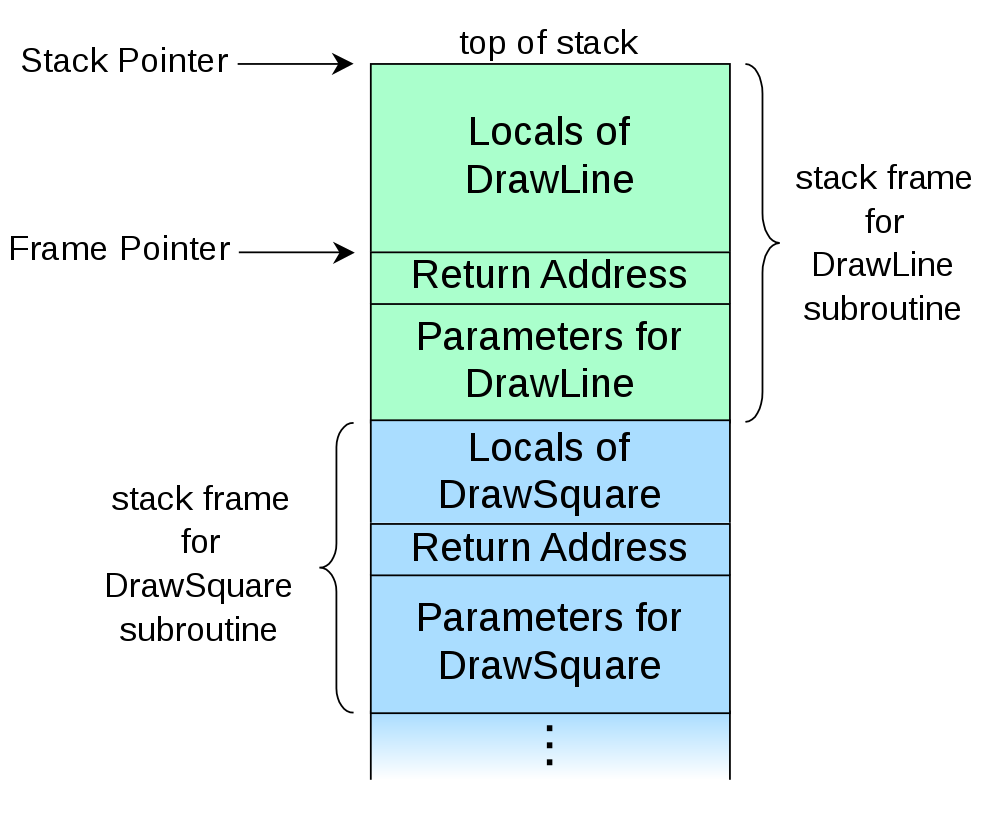
\includegraphics[width=.6\linewidth,keepaspectratio]{art/call-stack-layout.png}
	\caption{Call stack layout for downward-growing stacks\cite{online:stack-img}}
	\label{fig:call-stack-layout}
\end{figure}

The image also shows other important items for proper call stack operations. The \textit{stack pointer} (also in \autoref{fig:x86-regs}) is a CPU register that always points to the top of the stack, at the last accessible address. Another notable CPU register is the \textit{frame pointer}, or base pointer (\texttt{rbp}), which points at the base of the currently active stack frame. 

\subsection*{Accessing Thread Execution Stacks}
When using the usual \mintinline{c}|pthread_create()| API function, one simply has to provide a function as a parameter to create a new thread. Using the default parameters, this call makes the operating system allocate memory for the thread's stack, and then schedules it\cite{online:pthread-create}.

It is however possible for users of the POSIX threads library to specify a region of memory to use as stack space by specifying the attributes with \mintinline{c}|pthread_attr_setstack()|. This simple solution for thread stack execution access by BBPSim was thus chosen. Before starting any flight software thread, \gls{BBPSim} was modified to allocate 2MB of memory for it, which was considered to be sufficient for this application. It should be noted that this block of memory was required to be page-aligned to a virtual memory page. As a result, BBPSim held a reference to every thread's stack. It was then possible to include them in the checkpointing artifact, hence satisfying the third and last necessary condition for a stable restore.

\subsection*{Reconstructing Flight Software Threads}
Once the necessary components were saved as part of the first BBPSim simulation, both the fresh and mature threads had to be brought back in the same state as they were before. Nevertheless, the past execution stacks and register sets weren't enough, by themselves, to be able to restart the past threads. Some meticulous manipulations of that data had first to be done. 

Indeed, the reconstruction of flight software threads had to reconcile two different ecosystem together. From the operating system's point of view, the threads that were spawned in the second simulation run were completely different from those on the first. But from the flight software's perspective, the threads had to be, functionally speaking, the same. In that sense, one couldn't simply copy the old stack onto the new and expect the thread's execution to continue seamlessly. One reason for this is that important scheduling information was contained at the base of the stack, at higher addresses. 

To solve the problem, this thesis presents a way to reconstruct the old flight software threads by using new threads and meticulously replacing their stack frames with old frames. 

First of all, it was important to define the concept of \textit{user stack}. The stack of a pthread was divided in four main spaces, like \autoref{fig:stack-spaces} shows. The first two spaces were defined as containing all call frames pertaining to functions in the C and pthread libraries respectively, which use low-level Linux routines to coordinate the creation of the thread. As for the user stack space, it was defined as being the portion that contains all the frames related to \textit{user-defined functions}. In that sense, the \textit{user stack start} was defined as being located at the first 64-bit-aligned address after the pthread stack space. 
\begin{figure}[htbp]
	\centering 
	\includesvg[width=.8\textwidth]{svg/stack-spaces}
	\caption{Division of the execution stack into spaces.}
	\label{fig:stack-spaces}
\end{figure}

Because C code abstracts low-level constructs, finding the beginning of the user stack required the use of assembly. This was done by using \gls{GCC}'s inline assembly tools at the beginning of the first user function (the one provided to \mintinline{c}|pthread_create()|), as \autoref{code:usr-stk-start} shows\cite{online:inline-asm}. Once this address could be accessed, it was possible to deduce the total user stack start offset in any stack $s$ by subtracting the stack top's address:
\[
	\Delta_{usr}=s_{usr}-s_{top}
\]
Once this offset was obtained, it was crucial to include it in the checkpointing artifact, since pthreads don't necessarily \textit{always} have the same $\Delta_{usr}$. 
\begin{listing}[htpb]
	\centering
	\begin{minted}{c}
void bbpsimThreadEntry() {
	uint64_t x[4]; //0x20 bytes 
	asm volatile("mov %%rsp, %0  \n\t" //get current stack pointer
                 "addq $0x20, %0 \n\t" 
                 : "=r" (fswthread->m_pi8StartUserStack) //=$s_{usr}$
                 :);
	flightSoftwareTask(); //<- call never returns
}
	\end{minted}
	\caption{Capture of the user stack start.}
	\label{code:usr-stk-start}
\end{listing}

From then, it was possible to reconstruct the thread's execution stack the way it was before by copying only the user and unused portions of the old stack onto the new. This operation was done by the thread itself, using another inline assembly routine located in the restoring function. This stack-copying operation had to be done meticulously. It was important not to "pollute" the resulting stack, and thus this is why assembly was once again the perfect candidate. The ability to handle the registers manually could provide the required granular control. The complete thread reconstruction routine is included in \autoref{code:stk-copy-asm}. In the code, it is possible to observe many things. First, the \texttt{copyquadword} subroutine (at line \ref{code:copyqword-beg}) is called many times in order to copy the old user stack on the new one, starting from the correct offset. Then the routine jumps to \texttt{setcontext()}, which overwrites the current register set with the old one. This call should never return, because it sets the program counter to point back into the flight software code. Because \texttt{setcontext()} itself makes use of the stack\cite{online:setcontext}, it was important to first make the stack pointer point at an appropriate address, so as to not pollute the stack portions that were just written to. In the end, making a live thread replace its own stack frames could qualify as a careful stack corruption exercise, which is pictured in \autoref{fig:stack-reconstruction}.

\begin{figure}[htbp]
	\centering
	\begin{subfigure}{.33\linewidth}
		\centering\small
		\includesvg[height=\linewidth]{svg/stack-reconstruction1}
		\caption{Restored thread before}
	\end{subfigure}%
	\begin{subfigure}{.33\linewidth}
		\centering\small
		\includesvg[height=\linewidth]{svg/stack-reconstruction2}
		\caption{Old frames overwritten}
	\end{subfigure}%
	\begin{subfigure}{.33\linewidth}
		\centering\small
		\includesvg[height=\linewidth]{svg/stack-reconstruction3}
		\caption{Copy of the old frames}
	\end{subfigure}
	\caption{Stack reconstruction process.}
	\label{fig:stack-reconstruction}
\end{figure}

Keeping in mind that the \gls{BBPSim} library was always loaded at the same address, replacing the entirety of the new user stack by the old one had big benefits:
\begin{itemize}
	\item \textbf{Backtrace information was preserved}. This meant that, when using GDB to debug a restored simulation, the debugger would correctly find the return addresses in each stack frame (see \autoref{fig:call-stack-layout}) and could thus display the exact call stack that was just restored. The approach "fooled" GDB into thinking this new stack was there all along.
	\item \textbf{Stack variables were preserved}. With the way everything was copied over, even variables allocated on the stack would hold the same value. This meant that function-scoped variables could hold the same value as before.
\end{itemize}

Using this low-level approach, the restoring of a thread was near instantaneous, fulfilling customer requirement DCMS-BBP-56. The only cost was the stack-copying subroutine, which couldn't really be more optimized than the one in \autoref{code:stk-copy-asm}.

\subsection*{Solution Limitations}
Of course, using such a technique brought its lot of drawbacks. Since the old stack was copied integrally, this meant that stack-allocated pointers were put back as well, and thus held the same value as during the first simulation. In flight software, this was mitigated mainly for three reasons: 
\begin{enumerate}
	\item The address of static DAS variables was always the same, so those pointers would point to a valid address.
	\item Dynamic memory allocation wasn't used, so addresses were deterministic. BBPSim objects, though, were allocated dynamically, and some BBPSim-defined Deos types had to be modified to address the issue. This subject is treated in \autoref{cha:bbpsim-impl}. 
	\item The amount of old stack frames to copy back was low. This is because end-of-task-loop calls to \texttt{waitUntilNextPeriod()}, which checkpointed the flight software, were nearly always located in the task loop (i.e. when in the first user stack frame). This characteristic mitigated problems related to using the address of a function-local variable as a pointer parameter to another function, which would have been invalidated by the restoring process. 
\end{enumerate}

This process was also limited in the fact that the \texttt{-fomit-frame-pointer} GCC option unconditionally needed to be enabled. As the x86 architecture states, the frame pointer of the caller is usually pushed on the stack when calling a function\cite{online:x86-abi}. This means that the stack usually contains data that points inside \textit{itself}. As thread stacks were dynamically allocated, and thus were never located at the same place in memory, frame pointers were a big problem. Adding the GCC option when compiling every C and \Cpp file completely removed that limitation by taking out the reliance on the frame pointer entirely. It results in slight modifications to the compiled program, which changes the access to stack-allocated variables to be based on an offset from the \textit{stack pointer} rather than the frame pointer\cite{online:omit-frame-pointer}.

Finally, this solution was definitely not portable. Although this wasn't a problem for BBPSim, using the presented technique to cover a wide range of architecture in a general program would not work without extensively rethinking it. In addition, the use of inline assembly is compiler-specific. Even though GCC is very popular, this stack-copying approach is still locked to this compiler. 


%{
\setlength{\parindent}{2em}
\chapter{BBPSim Snapshotting}\label{cha:bbpsim-impl}
Previously, it was seen that the \gls{BBPSim} environment was composed of mainly three layers. The flight software was defined as its own layer, while the other two, the operating system and hardware layers, were built around the first one. In \autoref{cha:das-impl}, techniques for external access to flight software variables and execution structures were detailed. The main reason for this manipulation was that no code modification to the FSW was allowed. However, code in the BBPSim domain (OS and HW layers) did not suffer from the same constraint. 

In this chapter, the design and implementation of the checkpointing strategy of the BBPSim layers is described, along with some other potential solutions. An analysis of the necessary BBPSim data to package in the checkpointing artifact is first done. Then, details about the practical implementation are given along with the general architecture. Finally, the global performance of the save and restore feature is discussed and compared to the requirements. 

\section{Layer Analysis}
Saving the layers of the environment first requires one to broadly understand how BBPSim was designed in order to produce a quality solution tailored for its needs. In \autoref{sec:fsw-outline}, it was seen that, to offer a good ecosystem for the flight software's testing, \gls{BBPSim} reimplemented embedded operating system functionalities that were only available on the Deos \gls{RTOS}. Since the simulation framework was developed to run solely on the Linux platform, these functionalities had to be translated to use only available constructs. In parallel, the FSW also used the components present on the custom hardware designed for the Dream Chaser Communication Subsystem (called the \gls{BBP}). This required the simulator to emulate those behaviors as well.

In practice, every software or hardware utility that was mimicked was encapsulated in a child class of \texttt{CSimModule}. In BBPSim, a simulation module was represented as being an entity that can be initialized, processed at every step and resetted. \autoref{fig:os-layer} and \autoref{fig:hw-layer} present a brief summary of the general inheritance model of the modules. 
\begin{figure}[htbp]
	\vspace{12pt}
	\centering
	\footnotesize
	\includesvg[width=\linewidth]{svg/os-layer}
	\caption{Shortened UML class diagram of the operating system layer.}
	\label{fig:os-layer}
\end{figure}
\begin{figure}[htbp]
	\vspace{12pt}
	\centering
	\footnotesize
	\includesvg[width=\linewidth]{svg/hw-layer}
	\caption{Shortened UML class diagram of the hardware system layer.}
	\label{fig:hw-layer}
\end{figure}

Particularly in \autoref{fig:hw-layer}, it is possible to observe that the modules could also contain multiple child modules. Each object held data specific to the component it was simulating. This of course reflects the object-oriented concepts of the software, which was written in \Cpp.

This thesis argues that the BBPSim-domain modules and managers (from the OS and HW layers) all had specifically different data to backup in the checkpointing artifact. For example, when saving an ongoing simulation, the Mutex Manager must of course save the created mutexes up to the SAVE command, while the Bootstrap had to save where the simulation was located in its bootloading sequence. It is easy to see that a general strategy was needed in order to satisfy the many different types of data that could be saved. And with the tree-like design of BBPSim, the solution was required to also be flexible with its heuristic. 

\section{Checkpointing Strategy}
It was seen, in \autoref{cha:prod-artifact}, that the artifact produced by a checkpoint was decided to be made up of several record blocks chained together. This formatting approach was useful in this context, because it could clearly fragment data that belonged to various entities within the simulator, but still unify everything simultaneously. 

The way this data would be gathered and serialized in binary would still need to be resolved. Since this was object-oriented code, the general guideline was to keep everything encapsulated: each simulation module should know how to checkpoint itself. Practically, there were various possible implementation strategies to investigate:
\begin{itemize}
	\item \textbf{One RecordBlock interface, Overload input stream operator}. This is an easy saving mechanism. Every type of record block would have to be defined as its own class, that knows how to serialize itself in the binary checkpointing artifact using the input stream operator ("\texttt{< <}"). At saving time, the modules would create and fill their record blocks objects and serialize them inside the file. The serialization could have been done with the boost library\cite{online:boost}.
	
	This approach was considered too code-heavy. It relegated the responsibility of serialization to another object (instead of the simulation module itself), and the relationship between the module and the record block classes would have been too fuzzy. In addition, since the record blocks had to be tagged, measured and CRC'ed before getting written to file, this architecture did not produce an elegant solution. 
	\item \textbf{Define record blocks as nested classes within their modules definition}. This wasn't a good approach, because the quantity of different \gls{RB} was just too high. For instance, in \autoref{fig:hw-layer}, \texttt{CRiof} contained multiple submodules itself. This would have made the header files way too big. Not only that, the definition of record block would have been too similar with the module that would create them. 
	\item \textbf{Iterate the modules with a builder-like object}. This was the adopted solution. The builder object would expose a set of methods to the modules and let them organize their data to build their own record blocks, without having to define more types. At restore time, the inverse operation would be done with a different kind of object.
\end{itemize}

\subsection*{\Cpp Interfaces}
In that sense, the \texttt{CRestorableObject} interface was created. Every object that would want the ability to save and restore itself could implement the interface and organize its own checkpointing/restoring. This is depicted in \autoref{fig:rest-obj}. This solution followed one of the standard guidelines of object-oriented programming, which is, in this case, to encapsulate the behavior common to multiple types of objects. 
\begin{figure}[htbp]
	\centering
	\vspace{12pt}
	\footnotesize
	\includesvg[width=.6\linewidth]{svg/rest-obj}
	\caption{UML class diagram of the \texttt{CRestorableObject} interface.}
	\label{fig:rest-obj}
\end{figure}

From that point, a standard interface for saving and restoring was defined. When a SAVE command gets executed, a \texttt{CEnvironmentSaver} instance iterated through all the simulation modules and gathered the relevant data. At restore time, the \texttt{CEnvironmentRestorer} object would do the reverse operation. For both pure virtual methods, an pointer parameter could be specified. The addition of this parameter was justified by the tree-like design of the simulation modules. Since some modules could be instantiated multiple times (like \texttt{CRt1553} of \autoref{fig:hw-layer}), it was necessary for their owner to pass down an identifying value or object in order to differentiate them. The returned value specified whether the operation was successful, not successful or completed with warnings. 

Once the iteration process was defined, the \texttt{CEnvironmentSaver} class needed to fulfill the needs of the different simulation modules. The UML diagram of the class is given in \autoref{fig:env-saver} It was mentioned previously that the object was defined as being a building object. In the case of the checkpointing of the OS and HW layers, two different types of payload to be contained in a record block were defined: static and dynamic. 

\begin{figure}[htbp]
	\vspace{12pt}
	\centering
	\footnotesize
	\includesvg[width=.75\linewidth]{svg/env-saver}
	\caption{UML class diagram of the CEnvironmentSaver interface.}
	\label{fig:env-saver}
\end{figure}


Dynamic blocks were blocks created and built on-demand by the simulation modules, specifically when the \texttt{CEnvironmentSaver} was iterating them while gathering the RBs. Creating such a block was done by using a sequence of member functions together. The user had to first begin a block by specifying its type with \texttt{BeginBlock()}. The data could then be inserted into the record block with either \texttt{AddBytesToBlock()}, for adding raw bytes, or with the \texttt{AddToBlock()} template method, which could take any type of data as input. After adding everything necessary, the user would then call \texttt{EndBlock()}, which would finalize the block by calculating its CRC16 and adding it to the list of blocks pending to be written to file. An example usage of this implementation for the FIFO Manger is given in \autoref{code:env-saver-use}. One can see that once the necessary data is included in the block in progress, the Manager lets the FIFO queue save its own messages recursively, because it also inherits from \texttt{CRestorableObject}. This was once again done with the intent of encapsulating the classes.

The static record blocks, on the other hand, were defined as containing data that existed statically in memory during the entire checkpointing operation. One example of this type of block would be the content of the \texttt{.bss} and \texttt{.data} sections of the flight software. These RBs were not specifically built for the \texttt{SaveTo} method, because they already existed. Since they were contiguous ranges of memory, the DAS State Manager could make an entire record block out of these chunks of memory only by specifying their address. 

While the simulation modules were iterated over, all record blocks were built and gathered. To conclude the saving operation, \texttt{DumpToFile()} then wrote all the record blocks to the checkpointing artifact, along with the artifact header. It should be noted that, since there was no restriction on the amount or size of record blocks, each module could add as many record blocks as needed. This solution for gathering checkpoint data is akin to the one in \autoref{sec:virtualbox} (VirtualBox) where the modules also save themselves.

At restore time, a similar but reverse implementation was designed. This is reflected in the \texttt{CEnvironmentRestorer} class. When initializing a simulation, a \texttt{CEnvironmentRestorer} instance started by reading the header of the checkpointing artifact. This is where the current \pathmono{libBbpSim.so} loading address was validated, to make sure it was loaded at the same address as when the checkpointing artifact was produced. The restorer then read the record blocks, validated their CRC, and iterated through the simulation modules, which had to implement their own restoring sequence.

\begin{figure}[htbp]
	\vspace{12pt}
	\centering
	\footnotesize
	\includesvg[width=.75\linewidth]{svg/env-restorer}
	\caption{UML class diagram of the CEnvironmentRestorer interface.}
	\label{fig:env-restorer}
\end{figure}

The main focus of the \texttt{CEnvironmentRestorer} class was to organize the record blocks and make them easily accessible through a small set of methods. It was designed to be comparable to an implementation of the Iterator design pattern by providing a way to access the elements of the artifact sequentially without exposing the underlying representation\cite{misc:iterator-des-pat}. This is depicted in \autoref{fig:env-restorer}. When a module restores itself, it must first query for a certain type of block via the \texttt{QueryBlockType()} method. The module can then read any amount of a defined type from the block by using the \texttt{ReadFromBlock()} template method. This reading operation must be made in the same order as the saving, as \autoref{code:env-restorer-use} shows.

During the restoring operation, it was important for the simulation modules to know the size their related record blocks. Since the interpretation of bytes inside a record block was relegated to them, it was their responsibility to produce blocks of a predictable size. Therefore, a conditional addition to the record block, like the one below, was not permitted.
\begin{minted}{c++}
if(ptrToVariable != nullptr) {
	envSaver.AddToBlock(*ptrToVariable);
}
\end{minted}

As mentioned previously, the checkpointing strategy was designed as a global approach for the saving and restoring of the simulation modules in \gls{BBPSim}. Since every one of them had different data to checkpoint, each had to have a custom implementation fo the \texttt{CRestorableObject} interface. This solution was considered scalable, because adding in a new component would only mean implementing its saving and restoring methods.

\section{Checkpointed Items}
Knowing what to include in the checkpointing artifact was vital in ensuring a stable restoring sequence. Before saving everything, a simple recipe was put in place to identify which variables had to be saved. First of all, it was possible to divide a simulation into four distinct phases that happened in succession:
\begin{enumerate}
	\item \textbf{Resource creation}, when the allocation and construction of the simulation modules took place.
	\item \textbf{Modules initialization}, when the INIT command was sent (\mintinline{c}|module->Initialize()|).
	\item \textbf{Environment loading}, an \textit{optional} phase when the simulation environment (all the modules) got restored from a file.
	\item \textbf{Normal use}, when the user would be stepping BBPSim. 
\end{enumerate}

The process that was applied to every member variables/component of every module was simple. If the variable was set in phases 1 or 2, and then never rewritten, then there was no need to save it, since those steps were always executed in every simulation. If the variable was a pointer, the strategy to save it depended on the context, but usually the object being pointed was serialized and saved, since a pointer couldn't be saved because it would be invalidated in the future. As for simple data, like \texttt{struct}s and \gls{POD} variables, they were included byte-for-byte in the relevant record block.

By following this plan for every components, one could extract a description of the items saved by some important OS modules, like the one given in  \autoref{tab:sim-mods-save}. 

\begin{table}[H]
	\centering
	\ra{1.2}
	\begin{tabularx}{\linewidth}{l X}
		\toprule
		\textbf{Module} & \textbf{Items Saved}\\
		\midrule
		Boostrap & {General state of the booting sequence: current boot delay and countdown in steps}\\
		\midrule
		FIFO Manager & {For each user-created queue: ID, attributes and every message in the queue in the same order (see \autoref{code:env-saver-use})}\\
		\midrule
		Mutex Manager & {For each user mutex: ID and name.}\\
		\midrule
		Sem. Manager & {For each user semaphore: ID, name and state (count).}\\	
		\midrule
		Mailbox Manager & {Similar to the FIFO Manager, since mailboxes were implemented as 1-sized queues.}\\
		\midrule
		Scheduler & {For each flight software thread:
		\vspace{-6pt}
		\begin{itemize}\setlength\itemsep{0em}
			\item ID and name
			\item The task's function address (pointer)
			\item The execution stack and stack pointer placement information
			\item The threads CPU register set at the last checkpoint (see \autoref{sec:das-exec-restore})
		\end{itemize}	
		}\\
		\bottomrule
	\end{tabularx}
	\caption{Non-exhaustive list of items saved when executing a checkpoint.}
	\label{tab:sim-mods-save}
\end{table}

It is important to note, in the case of the mutexes, that their state (locked/unlocked) wasn't saved. At restore time, they would all be restored to be in the unlocked state. This was considered a better choice for two reasons: 
\begin{enumerate}
	\item Flight software tasks always acquired and released mutexes in the same task loop (i.e. from scheduling to calling \texttt{waitUntilNextPeriod()})
	\item Because \gls{BBPSim} used the pthread library in the background, mutexes of types \texttt{pthread_mutex_t} were used. Using this type of mutex requires the user to always release a mutex from the same thread as the one which acquired it. Otherwise, the specification mentions undefined behavior\cite{online:pthread-mutex}. This meant that the restored threads would have had to recreate the mutexes they themselves created in the previous simulation run. This was considered too complex to implement.
\end{enumerate}

In the end, with all the data gathered, the checkpointing artifact's size was of the order of 115MB. This size depended on many things, but the amount of threads running when saving was the biggest factor of variation.

\subsection*{File System}
To continue the serialization process, the content of the flight software's emulated file system also needed to be included in the checkpointing artifact. This was due to the operating system layer reimplementing an API to manipulate files located in the Linux machine's file system. On the actual \gls{BBP} hardware, this data was located in flash.

First, by using a Linux standard program, it was possible to zip the file tree, containing some binary files, into one archive that was serialized into a record block using the following command:
\begin{minted}{bash}
zip -r file/tree/root *.bin
\end{minted}
At restore time, the archive would be unzipped by a similar command and the file tree would be copied back or overwritten at the same location on the Linux machine.

Secondly, since the manipulation of files implied that the operations could span multiple simulation steps, the state of a possibly currently opened file was also included in the checkpointing artifact. At saving time, the file would be reopened and the position of the reading cursor within the file would also be restored. 

\subsection*{Shared Memory}
Finally, the content of the Shared Memory was considered very important to include in a checkpoint, since this object represented, to some degree, the state of various hardware communication modules. As mentioned previously, the Shared Memory was a user-allocated \texttt{struct} instance. As such, it was trivial to include the raw bytes in the checkpointing artifact.  

\section{Save \& Restore Performance}
In \autoref{sec:reqs}, it was mentioned that the save and restore feature was guided by many customer requirements. Some of these requirements concerned the general performance of BBPSim, which directly affected the implementation of the feature. Particularly, requirements DCMS-BBP-56 and DCMS-BBP-69 (see \autoref{tab:customer-reqs}) were the main reason for the entire feature's performance goals.

Chapter \ref{cha:das-impl} mentioned that the restoring of DAS threads was very fast. By using the \texttt{/usr/bin/time} Linux profiling tool, it was possible to quantify that metric at  850ms to 1 second on average, well below the 5 min imposed by DCMS-BBP-56. As for the memory usage of the BBPSim simulator, results using the same profiling tool for RAM indicated a maximum memory usage of a little bit more than 261MB when restoring, which also fulfilled requirement DCMS-BBP-69. The output can be seen in \autoref{app:ram-profiling}. 

A lot of the memory usage could be attributed to the handling of statically-allocated flight software variables, located in the \texttt{.bss} and \texttt{.data} sections. In \autoref{sec:das-mem-restore}, it was seen that these sections took up about 100MB of space in RAM. However, the RAM usage in \autoref{app:ram-profiling} showed a usage of more than two and a half times that amount. This was attributed to the fact that, at restore time, the checkpointing artifact got loaded, read and \textit{copied} into memory by the \texttt{CEnvironmentRestorer} before it iterated through all simulation modules. This meant that, during the restoring process, space was allocated for both the big record blocks and the real statically-allocated DAS variables at the same time. 

Another notable value included in \autoref{app:ram-profiling} is the number of page faults. By instrumenting the restoring code using the \texttt{valgrind} profiling tool's utilities, it was possible to see that a lot of cache misses happened during the reset of the DAS State Manager, as part of the restoring sequence (see \autoref{app:valgrind-profiling}). Cache misses are a non-desirable latency caused by the CPU accessing sections of RAM for the first time. Before being written or read, these blocks of memory must first be brought into the CPU's cache\cite{misc:cache-misses}. In BBPSim, the DAS State Manager module was responsible for copying back the content of the \texttt{.bss} and \texttt{.data} sections of the flight software into their real memory ranges. At restore time, these sections would get overwritten with a big \texttt{memset}. Since the computer didn't use those pages of the computer memory within the program's life up to the restoring time, the memory accesses caused a lot of page faults and cache misses that slowed down the feature's performance.

}
%\chapter{Conclusion and recommendations}\label{cha:conclusion}

}


% post-content of thesis
%\nocite{*} <- use this to list everything, even stuff not cited
\renewcommand{\bibname}{References}
\printbibliography

%\begin{appendices}
%{
\chapter{C Variables and their Segments}\label{code:c-to-segments}

\begin{minted}{c}
// main.c

/* statically-allocated variables       	*/
/* this means they exist for the entire 	*/
/* execution of the program             	*/
/* They all go in the .bss section 			*/
/* since uninitalized or init to 0 			*/
static int aVariable;//$\label{lc-beg-statics}$
static int anotherVariable = 0;
int aVariable;
int anotherVariable = 0;

/* constant, so defined in .rodata		 	*/
static const double pi = 3.1415;

/* statically-allocated variables       	*/
/* They all go in the .bss section 			*/
int anInitedVar = 42;
static int anotherInitedVar = 42;//$\label{lc-end-statics}$

/* Executable code, so defined in .text 	*/
int count() {
	static unsigned int theCount = 0; //also goes in .bss 
	return theCount++;
}
\end{minted}

\chapter{Mapping Produced by the Linker for BBPSim}\label{map:ld}

{\small
\begin{verbatim}
[... skipping output ...]

.das_state_vars_data
0x0000000000759a80      0x4f0
0x0000000000759a80                __das_state_vars_data_start = .
SORT(*obj/DasSrc/*.o)(.data .data.* .gnu.linkonce.d.*)
.data        0x0000000000759a80          0x0 obj/DasSrc/Common/src/APID.o

[... skipping output ...]

.data        0x0000000000759f40         0x30 [...]/src/RoutingProcessing.o
.data        0x0000000000759f70          0x0 [...]/src/StateHandler.o
0x0000000000759f70                __das_state_vars_data_end = .

.das_state_vars_bss
0x0000000000759f80  0x51b1068
0x0000000000759f80                __das_state_vars_bss_start = .
SORT(*obj/DasSrc/*.o)(.bss .bss.* COMMON)
.bss           0x0000000000759f80        0x0 obj/DasSrc/Common/src/APID.o
.bss           0x0000000000759f80        0x0 obj/DasSrc/Common/src/Crc16.o

[... skipping output ...]

.bss           0x000000000590a8e0      0x3b8 [...]/src/RoutingProcessing.o
*fill*         0x000000000590ac98        0x8 
.bss           0x000000000590aca0      0x348 [...]/src/StateHandler.o
0x000000000590afe8                __das_state_vars_bss_end = .
\end{verbatim}
}
\chapter{Sanitized List of DAS Variables}\label{das-symbol-catalog}

{\small
\begin{verbatim}
e6069e4f97d40996a8ea84bbb62eaf6b16aec786
0000000000759a80 0000000000000000 __das_state_vars_data_start
0000000000759a80 0000000000000004 m_u32DasSwTraceFilter
0000000000759aa0 0000000000000040 asTflLoadingOrder
0000000000759ae0 0000000000000020 asDidlLoadingOrder
0000000000759b00 0000000000000030 asIpclLoadingOrder
0000000000759b40 0000000000000001 m_u8PageReadCount
0000000000759b60 0000000000000054 m_u32BinaryFileSizeStatus
0000000000759bc0 0000000000000020 m_aeFileLoadStatus
0000000000759be0 0000000000000040 m_strBinaryFileList
0000000000759c20 0000000000000008 m_asExtCmdTlmSubsystem
[... skipping output ...]
0000000000759d10 0000000000000008 m_asRsVcduRxCntTlm
0000000000759d18 000000000000000c m_asFrameSyncMissCntTlm
0000000000759d24 000000000000000c m_asFrameSyncDetectCntTlm
0000000000759d30 000000000000000c m_asVcduTxCntTlm
0000000000759d3c 0000000000000008 m_asIdleFrameTxCntTlm
0000000000759d44 0000000000000008 m_asDataFrameTxCntTlm
0000000000759d4c 000000000000000c m_asPassThroughTxCntTlm
0000000000759d60 0000000000000016 m_au16CmdMsgTimeoutInMs
0000000000759d80 0000000000000020 m_sFtfcMemPool
0000000000759da0 0000000000000020 m_sGtwMemPool
0000000000759dc0 0000000000000120 m_asRfcuRffeReceiver
0000000000759ee0 0000000000000028 m_au8TimeSuitePerRate
0000000000759f08 000000000000000c m_au8C2v2RateToTimeConversion
0000000000759f20 0000000000000014 m_au8TdrsRateToTimeConversion
0000000000759f40 0000000000000030 mc_asVcidFtrList
0000000000759f70 0000000000000000 __das_state_vars_data_end
0000000000759f80 0000000000000000 __das_state_vars_bss_start
0000000000759f80 0000000000000004 m_bDasIntegrationTraceFilter
[... skipping output ...]

\end{verbatim}
}

\chapter{Symbol Cataloging Process}
\begin{figure}[H]
	\centering
	\includesvg[width=\linewidth]{svg/blackbox-diagram}
	\caption{Sequential steps to include the symbol catalog in \pathmono{libBbpSim.so}}
	\label{fig:blackbox-diagram}
\end{figure}


}
%\end{appendices}

\end{document}
